\documentclass[FrontPage]{grattan}

\title{All complications should count: Using our data to make hospitals safer}
\author{Stephen Duckett and Christine Jorm}
\hypersetup{pdftitle={All complications should count: Using our data to make hospitals safer},pdfauthor={Stephen Duckett and Christine Jorm and Lucille Danks and Greg Moran}}
\GrattanReportNumber{2018-01}
\addbibresource{./bib/lifting-the-lid.bib}


\providecommand*{\hl}[1]{\textcolor{red}{#1}}
\AtBeginEnvironment{quote}{\small\justifying}
\usepackage{longtable}
\DeclareMathOperator{\Var}{Var}

\urldef\coagURL\url{https://www.coaghealthcouncil.gov.au/Portals/0/COAG%20Health%20Council%20Communique%20-%204%20August%202017.pdf}

\newcommand*{\ShinyAppURL}{\textcolor{blue}{\url{https://grattan.shinyapps.io/all-complications-should-count/}}}
\newcommand*{\Figure}[1]{Figure~#1}

% add_to_dictionary: CHADx CHAPx underuse centredness multiday sameday ABO puerperium
% add_to_dictionary: perineal specialty specialties MCHA[PD]x[0-9]*
% add_to_dictionary: Belinda Dromana comorbidities gonarthrosis
% add_to_dictionary: Thrombophilia bariatric Roundtable grassroots
% add_to_dictionary: glycaemic BUPA Healthscope gastroplasty
% add_to_dictionary: biliopancreatic jujunal illeal postpartum SEIFA

% add_to_dictionary: multipurpose comorbidity Charlson Elixhauser Std
% add_to_dictionary: casemix Mundlak equi-correlation nonlinearities
% add_to_dictionary: Raphson nonlinear GLLAMM Stata regressors Bonferroni
% add_to_dictionary: Nonobstetric Epanechnikov wellbeing Hausman
% add_to_dictionary: detrend demeaned calc th Maj mgmt proc\. KR
% add_to_dictionary: proc

\usetikzlibrary{calc,decorations}



\acknowledgements{%
This report was written by Stephen Duckett, Grattan Institute Health Program Director, Christine Jorm, Honorary Fellow, and Lucille Danks and Greg Moran, Associates. Hugh Parsonage provided extensive assistance in the finalisation of this report.

We would like to thank numerous people from the health policy community including Ian Brownwood, Michael Daly, Irfan Dhalla, Jean-Frédéric Lévesque, Alison Verhoeven, John Wakefield, and Grattan Institute’s Health Program Reference Group for their helpful comments. 

The opinions in this report are those of the authors and do not necessarily represent the views of Grattan Institute's founding members, affiliates, individual board members, reference group members or reviewers.
Any remaining errors or omissions are the responsibility of the authors.

Grattan Institute is an independent think tank focused on Australian public policy.
Our work is independent, practical and rigorous.
We aim to improve policy outcomes by engaging with both decision-makers and the community.

For further information on the Institute's programs, or to join our mailing list, please go to: \textcolor{blue}{\url{https://www.grattan.edu.au/}}.

% editorial_author_only: Hugh Parsonage
% add_author_to_recommended_citation_at: Christine Jorm 2
{\footnotesize
This report may be cited as:
Duckett, Stephen, Jorm, Christine, Danks, Lucille, and Moran, Greg (2018). \emph{\mytitle}. Grattan Institute.

ISBN: 978-0-6482307-1-7

All material published or otherwise created by Grattan Institute is licensed under a Creative Commons Attribution-NonCommercial-ShareAlike 3.0 Unported License\par
}
}

\begin{document}

\begin{overview}
One in every nine patients who go into hospital in Australia suffers a complication -- about 900,000 patients each year.
If they stay in overnight, the figure rises to one in four -- about 725,000 patients each year.
A patient's risk of developing a complication varies dramatically depending on which hospital they go to: in some cases, the additional risk of a complication at the worst-performing hospitals can be four times higher than at the best performers.
If all hospitals lifted their safety performance to the level of the best 10 per cent of Australian hospitals, the complication rate across the nation would fall by more than a quarter.

This report exposes the flaws in Australian hospitals' safety and quality monitoring regime, and recommends reforms that could result in an extra 250,000 patients leaving hospital each year free of complications.

At the moment, a veil of secrecy hangs over which hospitals and clinicians have higher rates of complications and which are safety leaders.
Hospital safety statistics are collected, but they are kept secret, not just from patients but from doctors and hospitals.
This has to change.
Patients have a right to know the data on complication rates in different hospitals and for different procedures, so they -- and their GPs -- can make better-informed decisions about how and where they are treated.
Doctors and hospitals need to know how they are performing compared to their peers, so that they can learn from the best-performing hospitals and clinicians.

At the moment, hospital safety policies focus on only a small subset of complications classified by government as being `preventable'.
Instead policy should be directed towards reducing all complications to the best rate achievable.
This requires building up a comprehensive picture of patient outcomes, and understanding how some hospitals and clinical teams reduce all complications and achieve excellent outcomes.

Private health insurers should release the information they gather on private hospitals: reducing complication rates would mean quicker recoveries and lower premiums for their members.
State and territory governments should release detailed data on the performance of both public and private hospitals.
This data needs to show the whole gamut of hospital performance, from catastrophic but rare errors to less harmful but prevalent complications.
It should highlight the areas where there is a big gap between the best and worst performers.
Governments need to set ambitious goals for every hospital -- public and private -- to improve their safety and quality of care.
And they need to ensure the data is published widely so that patients and taxpayers can see which hospitals are improving and which are not.
\end{overview}

\contentspage


\listoffigures

\chapter{The harm done}\label{chap:the-harm-done}

If a friend or family member is going to hospital, we usually wish them luck.
Why? Because we know that sometimes, things go wrong.

Even in the best of hands, there is the risk that a patient's problem proves trickier to deal with than anticipated: treatments aren't effective, perhaps more radical surgery might be required, or they may be left with a long-term impairment after treatment.
Less acceptably, errors are made and care doesn't go according to plan.
Patients are harmed: they fall, receive a drug they are allergic to or, rarely, have the wrong limb operated on.
Reviews of hospital charts suggest `adverse events' occur in more than 10 per cent of hospital admissions in Australia (ranging across hospitals from 2.9 per cent to 16.6 per cent) and at least half are considered to have been preventable.%
	\footnote{\textcite{baines2015effective}.
	The range is partly attributable to methodological differences in the studies.}

Media reports focus on the most shocking cases: a cluster of baby deaths at Bacchus Marsh Hospital in Victoria,%
	\footcite{Duckett-Review-2016-Quality-assurance-in-Vic}
or a sponge left inside a patient at Poplars Private Hospital in Sydney.%
	\footcite{Courts-2011-SMH-Woman-to-sue-after-sponge-left-in-body}
But most unsafe care is less dramatic: an otherwise healthy patient contracting an infection after their operation, for example.%
	\footcite{Vincent-2016-Safer-Healthcare}
Often no one is quite sure how or when a complication happened -- but the patient still needs extra treatment or a longer stay in hospital.

Australians expect all hospitals to provide high-quality care.
They may be surprised to learn that some hospitals achieve much better results for a procedure than others, and that the chance of something going wrong differs depending on which hospital treats you.

Good quality care has many aspects (see \Vref{box:safety-is-one-component-of-high-quality-health-system}), and the perspectives of patients, clinicians and managers might differ as to how different aspects of quality ought to be given priority.%
	\footcite{Duckett-Ward-2008-Robust-performance-benchmarks}
However, all agree that a key dimension of quality is safety; avoiding harm to patients from the care that is intended to help them.

\begin{bigbox*}{Safety is one component of a high-quality health system}{box:safety-is-one-component-of-high-quality-health-system}
The \emph{quality} of care is the degree to which health services for individuals and populations increase the likelihood of desired health outcomes and are consistent with current professional knowledge.%
	\footcite{Runciman_2009}

The Australian Safety and Quality Framework for Health Care gives a vision for care that is: patient centred, organised for safety, and driven by information.%
	\footnote{See: \textcolor{blue}{\url{https://www.safetyandquality.gov.au/national-priorities/australian-safety-and-quality-framework-for-health-care/}}.}

The dominant quality assessment framework developed by the US Institute of Medicine lists six aims for the health care system:%
	\footnote{See: \textcolor{blue}{\url{https://www.ahrq.gov/professionals/quality-patient-safety/talkingquality/create/sixdomains.html}}.}

\textbf{Safe}: Avoiding harm to patients from the care that is intended to help them.

\textbf{Effective}: Providing services based on scientific knowledge to all who could benefit, and refraining from providing services to those not likely to benefit (avoiding underuse and misuse, respectively).

\textbf{Patient-centred}: Providing care that is respectful of and responsive to individual patient preferences, needs, and values, and ensuring that patient values guide all clinical decisions.

\textbf{Timely}: Reducing waits and sometimes harmful delays for both those who receive and those who give care.

\textbf{Efficient}: Avoiding waste, including waste of equipment, supplies, ideas, and energy.

\textbf{Equitable}: Providing care that does not vary in quality because of personal characteristics such as gender, ethnicity, geographic location, and socioeconomic status.

The framework makes some potential trade-offs explicit.
It places safety below quality.
But care that is not timely is unsafe, as is ineffective care.
In practice, the terms safety and quality are often used interchangeably.
\end{bigbox*}

This report proposes four reforms to reduce variation in complication rates and improve the safety of hospital care.
The rest of this chapter argues that we should measure all complications, not just some.
\Chapref{chap:australia-needs-to-set-more-ambitious-hospital-safety-targets} shows that hospitals and doctors need to have the information necessary to know where they need to improve.
\Chapref{chap:data-can-inform-hospitals-about-their-specific-strengths-and-weaknesses} suggests that Australia should set a bold ambition: to reduce complication rates by more than a quarter of the current rate.
\Chapref{chap:we-need-to-share-data-openly} shows why there should be regular public reporting of the progress of each state and each public and private hospital toward this ambitious goal.

This chapter shows how a narrow view of safety has resulted in limited measurement of complications.
Safety monitoring should move away from a focus on errors to a more panoramic view of patient outcomes.

\section{One in nine patients suffer in-hospital harm}\label{sec:one-in-nine-patients-suffer-in-hospital-harm}

\begin{figure}[!t]
\caption{Complications are common}\label{fig:1-1-complications-are-common}
\units{Share of admissions involving at least one complication, per cent}
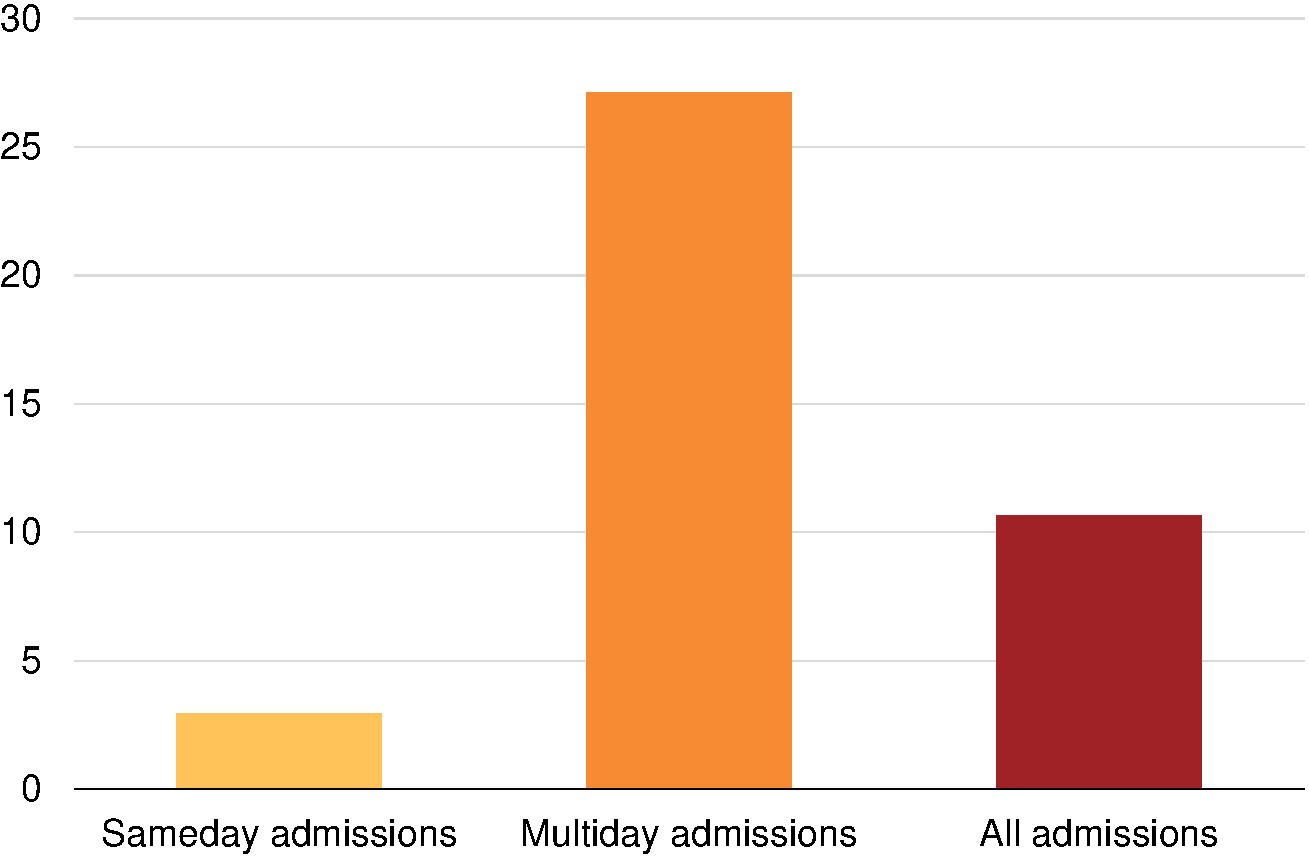
\includegraphics[page=1]{atlas/comps_charts.pdf}
\source{Grattan analysis of the 2012-15 National Hospital Morbidity Dataset}
\end{figure}

\begin{figure}[!t]
\caption{Procedural complications increase a patient's stay in hospital}\label{fig:1-2-avg-risk-adjusted-len-of-stay-for-patients-with-without-procedural-complications}
\units{Average length of stay (days)}
\includegraphics[page=18]{atlas/comps_charts.pdf}
\source{Grattan analysis of the 2012-15 National Hospital Morbidity Dataset}
\end{figure}

Over 2012-13 to 2014-15, one in every nine people admitted to hospital in Australia developed a complication.%
	\footnote{That is, an additional diagnosis was made that was not present when the patient went into hospital.
	The diagnosis may be quite serious or it may be of less consequence and may not even delay discharge from the hospital (though it must have been treated to be included in this data).
	A patient might have multiple complications across separate categories in the Classification of Hospital Acquired Diagnoses (CHADx+): \textcite{jackson2009classification}.
	All analyses in this report are based on patients classified as `acute' in the National Hospital Morbidity Dataset; see the Methodological Supplement for more details of the data set and our analytical approach, including how we standardise for patient factors.}
For patients who were in hospital overnight, the rate was even higher: more than one in four (\Vref{fig:1-1-complications-are-common}).
About 900,000 patients each year have a complication.%
	\footnote{About 725,000 overnight patients suffer a complication.}


These complications are a real problem.
Some cause patients discomfort, delay recoveries, and extend hospital stays.%
	\footnote{While many complications result in longer hospital stays, it is also true that more complex patients have longer stays, increasing their risk of complications such as infections.
	\Cref{fig:1-2-avg-risk-adjusted-len-of-stay-for-patients-with-without-procedural-complications} focuses on procedural complications. Unlike medication errors, the risk of procedural complications does not increase one-for-one with the length of a patient's stay.}
The most serious cause permanent injury or death.

On average, patients who suffer a complication after a procedure%
	\footnote{Defined as Major CHADx Class 1: Procedural complications.
	The CHADX+ classification system is described in \Cref{subsec:classification-of-hospital-acquired-diagnoses-chadx-or-all-complications}.}
end up staying in hospital for five extra days.
\Vref{fig:1-2-avg-risk-adjusted-len-of-stay-for-patients-with-without-procedural-complications} shows how this impact varies for two procedures, and for all overnight patients, other than women admitted to give birth.
Patients may continue to suffer the consequences of these incidents after they are discharged.

The following sections describe the evolution of a scientific literature on hospital safety as clinicians and managers doggedly chased better results for patients.



\section{The old way of thinking about safety normalised harm to patients}\label{sec:the-old-way-of-thinking-about-safety-normalised-harm-to-patients}

Over the past 40 years the health care system has moved from a focus on doctors' mistakes toward an understanding that poor outcomes are often the result of system rather than individual failures.
The publication of a landmark US report, `To err is human', in the year 2000 drew attention to the large amount of harm caused by health care and promoted a `systems approach'.%
	\footcite{NAP-2000-Err-is-human}
This led to an emphasis on `learning from mistakes', and trying to ensure that the culture of health services was just and facilitated that learning.%
	\footcites{Marx-2001-Patient-safety-primer-for-Health-execs}{Waring_2015}


\begin{verysmallbox}{Preventing the `unpreventable'}{box:preventing-the-unpreventable}
On occasions, system changes that eradicate certain types of `unpreventable' incidents have been identified.
For example, central line-related bloodstream infections in intensive care units were not considered `preventable' until a determined improvement and measurement effort in Michigan intensive care units proved otherwise.%
	\footcites{pronovost2010sustaining}{dixonwoods2012challenges}
\end{verysmallbox}

Yet safety was still defined as an absence of specific negative events.
When such events happened, there was a search for who or what caused the errors.
Such thinking inspired the development of health care incident reporting systems modelled on aviation safety reporting systems.
The hope was that the process of reporting, investigating, and determining how an event could have been prevented, and then changing systems, would make hospitals safer.%
	\footnote{The limitations of incident reporting systems are discussed in detail in the Grattan Institute's previous report, \citetitle{DuckettEtAl-2017-Strengthening-safety-statistics}.}

But this focus on preventability was misguided in several respects.
Most fundamentally, `preventability' was not a useful concept because what is `preventable' is subjective, changes over time, and depends on the context of care (see \Vref{box:preventing-the-unpreventable}).%
	\footcite{Vincent-2016-Safer-Healthcare}


Disagreement among clinicians about what should be considered `preventable' mired safety improvement efforts in an unproductive debate.
The concept of preventability also established a culture of blame.%
	\footnote{A leading Australian safety expert and a reviewer of this paper noted: ``Despite significant efforts over more than a decade, I and others have not been able to de-couple the notion of safety with `medical mistakes'.''}
This limited learning because it engendered defensiveness among those involved in safety incidents, and quests for root causes distracted from lessons that could be applied more generally.%
	\footcites{Cook-Nemeth-2010-Those-found-responsible-have-been-sacked}{hayward2001estimating}{Shojania541-Temporal-trends-in-patient-safety-Netherlands}{Vincent-2016-Safer-Healthcare}
Detailed investigations of rare, dramatic health care events have identified few patterns in the circumstances in which they arise, and so, unsurprisingly, have led to little progress in reducing their prevalence.%
	\footcites{Wears-2016-our-basic-premises-hidden-assumptions}{kellogg2017current}

But the most serious consequence of the focus on preventability was that it normalised harm to patients.
Focusing safety improvement efforts on `errors' that caused `preventable' harm implied that other instances of harm to patients were acceptable, and less worthy of being tackled.

Some clinicians routinely achieve better outcomes for patients than most.
For instance, elderly, obese patients with renal failure are at high risk of physiological deterioration, such as acquired fluid and electrolyte disturbances or pneumonia.
These complications may occur without any errors being made by clinicians, and, in some patients, the complications may be inevitable.
Yet some clinicians deliver care that beats the odds.

Focusing on only a subset of complications is a problem because it removes the impetus to innovate and learn from clinicians who manage, through clinical excellence, to defy the odds across a broad range of potential complications.

\subsection{New definitions of hospital safety focus on opportunities to improve}\label{subsec:new-definitions-of-hospital-safety-focus-on-opportunities-to-improve}

Safe care is now understood to mean more than ensuring no egregious errors occur -- it means ensuring that every patient's recovery is as swift and comfortable as possible.

The new emphasis is on reducing risk by improving system performance overall.%
	\footcites{Hollnagel-2014-Safety-Management}{Besnard2014}{DEKKER2014348}
This requires studying frequent events, and normal (and excellent) performance.
Safety monitoring needs to include the full spectrum of patient outcomes.
The aim is to ensure that the number of good outcomes is as high as possible and the number of events that could be harmful to patients is acceptably low.%
	\footnote{\textcite{Hollnagel-2014-Safety-Management}.
	It is also recognised by safety academics that even egregious errors such as incorrect site surgery will recur (\textcite{pandit2016deaths}).
	The concept of a `never event' is fundamentally flawed for a complex system like health care (\textcite{moppett2016surgical}), although attention to the processes of care can reduce the likelihood of an undetected error causing harm.}

\subsection{New definitions of hospital safety put patients at the centre}\label{subsec:new-definitions-of-hospital-safety-put-patients-at-the-centre}
Patients' priorities and experiences are now considered to be central to the safety of hospital care.%
	\footcites{jorm2009should}{hor2013finding}{pronovost2017creating}

This means safety improvement policies should acknowledge and facilitate patients' right to be informed about the likely outcomes of their care.%
	\footcite{Rubin-2017-Patient-empowerment}
It is now possible for a hospital to know the rate of complications which occurred for a patient in a given demographic having a given procedure in the past year.
Patients should know that information too, so they can appreciate the risks they face.%
	\footcite{Stacey_2017}

`Patient centredness' also means patients should be engaged in key decisions about their care.%
	\footnote{Patient decision aids, where used, improve patients' knowledge (\textcites{Stacey_2017}{Brown_2015}).
	Patient decision aids have been developed for many conditions (see: \textcolor{blue}{\url{https://decisionaid.ohri.ca/index.html}}), and the Australian Commission on Safety and Quality in Health Care has a program of work on patient decision aids (see: \textcolor{blue}{\url{https://www.safetyandquality.gov.au/our-work/shared-decision-making/patient-decision-aids/}}).
	However, patient decision aids have a number of limitations (\textcite{Agoritsas_2015}), not least of which is their implementation and use in practice (\textcite{Elwyn_2008}).}
Too often, only lip service is paid to `patient centredness'.%
	\footcites{lgar2014twelve}{stiggelbout2015shared}
While relatively few decision-making aids have been developed to engage patients in clinical decisions,%
	\footnote{A good exception is the wealth of decision-making aids available for breast cancer treatments.} sometimes clinicians may not have enough information to know the facts about risks and benefits themselves.
Consequently, they frequently overestimate benefits and underestimate risks.%
	\footcite{hoffmann2017clinicians}
This lack of -- or inaccurate -- information hinders proper informed consent.%
	\footnote{Medical practitioners always need to consider individual patient circumstances and their own experience, but we argue that relevant information often does exist and should be made available to consumers and practitioners.}
As one consumer argued recently:

\providecommand{\dictaline}{\textemdash}
\hyphenpenalty=100
\begin{quote}
One of the reasons that clinicians struggle to form partnerships with patients and consumers is that there is inadequate information for proper informed consent.
The numbers that are collected don't filter through to clinicians dealing with the patient, and certainly not to the patient themselves.
I encourage people to ask doctors three questions: `What are my options?', `What are the treatment outcomes -- both benefits and risks?', and `How likely are those outcomes to happen to me?'.
Doctors though say `We just don't have that information'.\\[-0.5\baselineskip]\null	\hfill\dictaline\ \textcite{Carey-2017-SPHERE}\par
\end{quote}
\hyphenpenalty=400

The shift toward patient centredness furthers, rather than competes with, clinical objectives.
When data about patients' likely outcomes is made public, clinicians evaluate the benefits and risks of care more accurately.%
	\footcite{sacks2016impact}
When patients are more engaged in shared decision-making, they gain a more accurate appreciation of the risks involved,%
	\footcite{Stacey_2017}
and become more comfortable with the decisions made and more satisfied with their care.%
	\footcites{boss2016shared}{walsh2014undetermined}{Stacey_2017}
They also suffer fewer adverse events.%
	\footcites{schiffinger2016two}{holzmueller2012framework}{Weingart-etal-2011-Patient-participation}



\begin{figure}
\caption{In Australia the rate of complications is not falling}\label{fig:1-3-rate-of-complications-not-falling}
\units{Share of admissions involving at least one complication, categorised by the most common CHADx+ categories, per cent}
\includegraphics[page=2]{atlas/comps_charts.pdf}
\note{Rates of individual CHADx+ categories have been scaled such that they sum to the share of admissions involving at least one of any complication.}
\source{Grattan analysis of the 2012-15 National Hospital Morbidity Dataset}
\end{figure}

\section{Australia's safety improvement efforts are yet to reflect these changes to safety thinking}\label{sec:australias-safety-improvement-efforts-are-yet-to-reflect-these-changes-to-safety-thinking}

Despite these substantial changes in the way experts are thinking about safety improvement, in Australia preventability is still the key criterion used, patients don't receive the information they could about risks and outcomes, and the data sources available to support safety improvement are not fully utilised.

In our previous report, \citetitle{DuckettEtAl-2017-Strengthening-safety-statistics}, sources of data on patient outcomes examined included: routine data, clinical quality registry data, death audit data, incident reporting and investigation data, patient-reported experience measures, and patient-reported outcome measures. Many instances were found where the data could and should be more accurate and relevant, and importantly more accessible and understandable. 

Incremental safety improvement efforts by clinicians are obstructed where there is limited transparency of data. Such limited transparency was justified only when there was a real threat of misplaced blame.%
	\footcite{DuckettEtAl-2017-Strengthening-safety-statistics}

Given this, it's unsurprising that Australia appears to be making negligible measurable progress on reducing the incidence of complications in hospitals.
\Vref{fig:1-3-rate-of-complications-not-falling}
shows that the prevalence and mix of complications in Australian hospitals didn't change significantly between 2012 and 2015.

This lack of measurable progress on this broad outcome measure might be a measurement problem that disguises an improvement trend: perhaps hospitals are becoming safer (as a result of a raft of State and National initiatives) -- but hospitals are also treating sicker patients overall.
However, there is little evidence of this latter trend.
The lack of overall improvement is especially disappointing when the `January effect' demonstrates that temporary organisational dysfunction results in measurable worsening of complications.%
	\footnote{\Cref{fig:1-3-rate-of-complications-not-falling} illustrates this `January effect' -- an uptick associated with transitions in hospitals over summer and at the start of a new year.
	Patients have longer stays, higher mortality and suffer from more adverse events in the month after
	 the mass changeover of junior medical staff and commencement of work by new, inexperienced interns:
	 \textcites{young2011july}{jen2009early}{wen2015july}.
	This period of significant organisational disruption happens in July in the US, August in the UK, and January in Australia, and hence is named differently.}
It's not unreasonable to expect improvements in hospital function and patient safety to have a measurable impact, gradually reducing the rate of complications.

To reduce the harm caused to patients, Australia needs to modernise its hospital safety improvement strategy.
The emphasis needs to \linebreak\vfill\null\eject
move away from analysing in excruciating detail where things went wrong,%
	\footnote{The limitations of the current reporting and investigation systems are discussed in \citetitle{DuckettEtAl-2017-Strengthening-safety-statistics}.}
and towards understanding how some clinical teams achieve exceptional outcomes; from a focus on blame to a focus on incremental improvement.

This report uses a powerful dataset to show how much scope there is for hospital safety to be improved.
In the tradition of Florence Nightingale, we focus on the rates and patterns of complications -- the epidemiology of patient outcomes.%
	\footcite{Florence-1999}

We take the position that it doesn't matter whether these complications have been declared to be `preventable' -- the fact that some hospitals consistently achieve much lower (risk-adjusted) rates than others is enough to demonstrate that there is scope for the incidence of all of these complications to be reduced.
Accordingly, we call for relative, rather than absolute, safety improvement goals -- a focus on \emph{reducing} all complications to the best rate achievable, rather than just focussing on \emph{preventing} some complications.

This report reveals the current variation in the safety of hospital care in Australia, and calls for a new national commitment to making all hospitals as safe as the safest 10 per cent.
It's an ambitious goal: it would reduce the national complication rate by more than a quarter.


\chapter{Australia needs to set more ambitious hospital safety targets}\label{chap:australia-needs-to-set-more-ambitious-hospital-safety-targets}

A lot of effort and expense is devoted to monitoring the safety and quality of care in Australian hospitals, but we are neither using the information as well as we should,%
	\footnote{As outlined in \citetitle{DuckettEtAl-2017-Strengthening-safety-statistics}.}
nor focussing on the right improvement targets.
This chapter argues for a more ambitious approach.

Indicators that assess quality of care have proliferated.%
	\footcite{copnell2009measuring}
Data and indicators are not the problem.
Australia has enough data to gauge the scope for improvement in hospital safety, using the same data that the Commonwealth Government uses to allocate funding to states for increases in hospital admissions and states use to determine hospital funding.%
	\footnote{This is not to say the data is perfect.
	Indeed we have identified areas where it should be improved (\textcite{DuckettEtAl-2017-Strengthening-safety-statistics}),
	 but coding of the data set has been shown to be reliable (\textcite{Henderson_2006}) and is regularly audited by states.}
The following sections describe the main measures of patient harm that are tracked for all hospital admissions, and compares them to reveal the lack of ambition in Australia's current safety monitoring policies.

\begin{table}
\caption{Far more harm is caused to patients in hospital than is captured in sentinel events or `Hospital Acquired Complications' statistics}\label{tbl:prop-admissions-with-geq-1-complication}
\units{Share of admissions involving at least one complication}
\begin{tabularx}{\linewidth}{p{0.35\linewidth}XX>{\raggedright\arraybackslash}X}
\toprule
\textbf{Complication type} & \textbf{Sameday admissions} & \textbf{Multiday admissions} & \textbf{All admissions}\tabularnewline
\midrule
{Sentinel events} & -- & -- & 0.0012\%\tabularnewline
\phantom{.} \\[-20pt]
{Designated `Hospital Acquired Complications' (HACs)} & 0.1\% & 5.2\% & 1.7\%\tabularnewline
\phantom{.} \\[-20pt]
{All complications} & 3.0\% & 27.1\% & 10.7\%\tabularnewline
\bottomrule
\end{tabularx}
\notewithsource{The shares of sameday and multiday admissions involving a sentinel event are not published and cannot be inferred from our dataset}%
{Grattan analysis of the 2012-15 National Hospital Morbidity dataset and the \textcite{PC-2017-Report-on-Govt-services--Public-hospitals}}
\vspace{2\baselineskip}
\null
\end{table}

\section{Australia has three key measures of unsafe care}\label{sec:australia-has-three-key-measures-of-unsafe-care}

Australia has three major classifications of harm to patients:
eight sentinel events, 16 priority `Hospital Acquired Complications' (HACs), and the comprehensive Classification of Hospital Acquired Diagnoses (CHADx+).%
	\footnote{The Annual Report on Government Services uses another classification set, but this is not used elsewhere (\textcite{PC-2017-Report-on-Govt-services--Public-hospitals}).}



\Vref{tbl:prop-admissions-with-geq-1-complication} shows the rates of the different types of complications. The rates equate to about 100 sentinel events recorded each year, about 140,000 priority Hospital Acquired Complications, and almost 900,000 complications of any kind.

Since 2002, Australia has had an agreed-upon list of eight extremely serious complications that are publicly reported.
This list was developed from one initially created as part of hospital accreditation in the United States in the late 1990s.%
	\footcites{Kizer-Stegun-2005}{Leape_2002}{Berman_1998}
Since then the US list has been revised multiple times.
It now has 29 items, which are now called `serious reportable events'.%
	\footnote{See: \textcolor{blue}{\url{http://www.qualityforum.org/Topics/SREs/List_of_SREs.aspx}}.}

\begin{smallbox}{Australia's eight sentinel events}{box:Aust-8-setinel-events}
\begin{enumerate}
\item Procedures involving the wrong patient or body part, resulting in death or major permanent loss of function
\item Suicide of a patient in an inpatient unit
\item Retained instruments or other material after surgery requiring re-operation or further surgical procedure
\item Intravascular gas embolism resulting in death or neurological damage
\item Haemolytic blood transfusion reaction resulting from ABO incompatibility
\item Medication error leading to the death of a patient reasonably believed to be due to incorrect administration of drugs
\item Maternal death associated with pregnancy, birth and the puerperium
\item Infant discharged to the wrong family
\end{enumerate}
\end{smallbox}

Australia's eight sentinel events are all catastrophic (\Cref{box:Aust-8-setinel-events}).
Fortunately, they are also rare: only 99 sentinel events were recorded across Australia in 2014-15.%
	\footcite{PC-2017-Report-on-Govt-services--Public-hospitals}
	Most of the listed events are likely to involve preventable errors.
But not all: maternal death is not always preventable, nor is intravascular gas embolism.%
	\footnote{We understand that removal of the some of the non-preventable events from this list may be imminent.}

\subsection{Hospital Acquired Complications (HACs)}\label{subsec:hospital-acquired-complications-hacs}

The HACs list, released in 2016, was developed as a subset of codes originally used in the Classification of Hospital Acquired Diagnoses (see next section). \Vref{tbl:incidence-of-hospital-acquired-complications} shows the incidence of HACs.

The HACs list was developed with a focus on preventability to be used for top-down accountability and funding.
Heads of government then agreed that the designated HACs met the following criteria:

\begin{itemize}
\item
  Clinical evidence is available to demonstrate that the HAC can be prevented with `best clinical practice'.
\item
  Evidence shows that individual hospitals and Local Health Networks are able to prevent the HAC and that the causes of the condition are within the control of the hospital.
\item
  The strength of external influences (\eg~patient factors) does not unduly affect the hospital's ability to avoid the HAC.
\item
  There is sufficient evidence to inform / instruct health services on how to avoid the HAC.
\item
  The development of the HAC measure has been subjected to valid construction.%
	\footcite{COAG-2017-ScheduleI-Revised-public-hospital-arrangements}
\end{itemize}

The Australian Commission on Safety and Quality in Health Care, which was responsible for the development of the HACs list, adopts a softer phrasing than the government position, stating that:

\begin{quote}
A hospital-acquired complication (HAC) refers to a complication for which clinical risk mitigation strategies may reduce (but not necessarily eliminate) the risk of that complication occurring.%
	\footnote{See: \textcolor{blue}{\url{https://www.safetyandquality.gov.au/our-work/indicators/hospital-acquired-complications/}}.}
\end{quote}

This softer phrasing is at odds with the use of the HACs list by the Commonwealth to adjust funding to states.
The state penalty varies with the complexity of the patient but for low complexity patients it assumes that 
all HACs can be prevented and so the state is to be penalised for the full incremental cost of the HAC.%
	\footcite{IHPA-2017-Risk-adj-model-tech-specs}

\begin{table}
\caption{Incidence of Hospital Acquired Complications, 2012-15}\label{tbl:incidence-of-hospital-acquired-complications}
\units{Share of admissions involving at least one complication}
\begin{tabularx}{\linewidth}{lXr}
\toprule
HAC1 & Pressure Injury                                              & 0.04\%\tabularnewline
HAC2 & Falls resulting in fracture or other intracranial injury     & N/A\tabularnewline
HAC3 & Healthcare associated infection                              & 0.76\%\tabularnewline
HAC4 & Surgical complications requiring unplanned return to theatre & N/A\tabularnewline
HAC5 & Unplanned intensive care unit admission                      & N/A\tabularnewline
HAC6 & Respiratory complications                                    & 0.08\%\tabularnewline
HAC7 & Venous thromboembolism                                       & 0.05\%\tabularnewline
HAC8 & Renal failure                                                & 0.01\%\tabularnewline
HAC9 & Gastrointestinal bleeding                                    & 0.09\%\tabularnewline
HAC10 & Medication complications                                    & 0.15\%\tabularnewline
HAC11 & Delirium                                                    & 0.30\%\tabularnewline
HAC12 & Persistent incontinence                                     & 0.05\%\tabularnewline
HAC13 & Malnutrition                                                & 0.07\%\tabularnewline
HAC14 & Cardiac complications                                       & 0.45\%\tabularnewline
HAC15 & Third and fourth degree perineal laceration during delivery & 0.08\%\tabularnewline
HAC16 & Neonatal birth trauma                                       & 0.00\%\tabularnewline
\multicolumn{2}{l}{Any HAC}                                       & 1.72\%\tabularnewline
\bottomrule
\end{tabularx}
\source{Grattan analysis of the 2012-15 National Hospital Morbidity Dataset.}
\end{table}

\subsubsection{HACs ignore some patients}\label{subsubsec:hacs-ignore-some-patients}

The HACs list excludes complications which occur in patients admitted for mental illness or who have drug or alcohol problems.
Yet these patients are not excluded from any other hospital-wide measure of the safety of care.

As illustrated in \Vref{tbl:mental-health-patients-also-experience-complications}, these patients also suffer complications in the HAC list. There is no legitimate reason to exclude complications occurring in patients with a principal diagnosis of mental illness or alcohol and drug conditions from system-wide monitoring.

\begin{table}
\caption{Mental health patients and drug and alcohol patients also experience complications}\label{tbl:mental-health-patients-also-experience-complications}
\units{Share of admissions involving at least one complication, by patient type}

\begin{tabularx}{\linewidth}{lRRRR}
\toprule
                  & Mental health patients & Drug and alcohol patients & Other patients & All patients\tabularnewline
\midrule
HACs              & 0.8\%                  & 0.4\%                     & 1.8\%          & 1.7\%\tabularnewline
All complications & 6.9\%                    & 4.7\%                       & 10.8\%         & 10.7\%\tabularnewline
\bottomrule
\end{tabularx}
\source{Grattan analysis of the 2012-15 National Hospital Morbidity Dataset}
\end{table}

\subsubsection{HACs ignore many complications}\label{subsubsec:hacs-ignore-many-complications}

The complications chosen for inclusion in the HACs list are somewhat idiosyncratic.
\Vref{fig:many-important-complications-are-not-included-in-hacs} shows that there is little consistency in the types of conditions included, nor in the narrowness with which conditions are defined.

The complications excluded from the list include serious complications, such as lacerations during procedures, and common complications with effective clinical risk mitigation strategies,%
	\footnote{That is, their prevalence can be reduced by appropriate drugs.}
such as constipation.
The HACs classification also defines some complications narrowly, such as acute renal failure and pressure ulcers, while applying no threshold at all for delirium, a common complication especially in dying patients.\footcites{oregan2013delirium}{hosie2013delirium}{grassi2015management}

\subsubsection{Improvements in small areas don't show up in the big picture}\label{subsubsec:improvements-in-small-areas-dont-show-up-in-the-big-picture}

Because HACs focus on a subset of complications, which don't occur with a high frequency, improvements in rates may not be seen when looking at complications overall.

There have been measurable improvements in the safety of hospital care in Australia in recent years.
For example, cases of \emph{Staphylococcus aureus bacteraemia} have declined from 0.96 to 0.73 cases per 10,000 days of patient care over the last four years, but because the number of cases involved is less than 1,500 in any year, this improvement is not picked up in looking at broad trends.%
	\footcite{AIHW-2017-Admitted-patient-care-2015-16-Aust-hosp-stats}
The same issue affects other HAC indicators.

\begin{figure}
\caption{Many important complications are not included in HACs}\label{fig:many-important-complications-are-not-included-in-hacs}
\units{Share and annual number of admissions involving at least one complication, classified by inclusion in the HACs priority complication list, per cent}
\includegraphics[page=4]{atlas/comps_charts.pdf}
\source{Grattan analysis of the 2012-15 National Hospital Morbidity Dataset}
\end{figure} 

\subsection{Classification of Hospital Acquired Diagnoses (CHADx+) or `all complications'}\label{subsec:classification-of-hospital-acquired-diagnoses-chadx-or-all-complications}

The CHADx+, first developed in 2009,
	\footcite{jackson2009classification}
aims to provide a comprehensive classification of all hospital-acquired complications present in the routine data (as recorded in the clinical record).
It has been revised a number of times and now also includes incidents detected using procedure codes (CHAPx).%
	\footnote{We use CHADx+ version 1.4 in this report.}

The CHADx+ classification does not flag which types of complications should be the focus of prevention initiatives.
It was designed to assist bottom-up improvement initiatives by local clinicians, by enabling hospitals and hospital departments to identify the complications relevant to their situation.
CHADx+ is publicly available, but used in only a few hospitals.

\Vref{tbl:incidence-CHADx} shows the overall incidence of CHADx+ complications, and the incidence of each major CHADx+ class.%
	\footnote{These estimates differ slightly from those published by the Australian Institute of Health and Welfare because this report uses a later, more comprehensive edition of the classification.
	For further details, see the Methodological Supplement to this report.}
Information on the most common complications for elective procedures -- categorised into CHADx+ classes and stratified by age, sex, and whether or not the patient stayed overnight -- is provided for each specialty at: \ShinyAppURL{}. This app provides a `proof-of-concept' as to the type of reporting that existing data sources allow.\footnote{At the time of publication, the app was still being refined. As such, results produced by the app should be taken as indicative only and not relied upon.}  

\begin{table*}
\caption{Incidence of CHADx+, 2012-15}\label{tbl:incidence-CHADx}
\units{Share of admissions involving at least one complication}
\begin{tabularx}{\linewidth}{lRlR}
\toprule
MCHADx1 Procedural complications              & 1.25\% & MCHAPx1 Ventilatory support                             & 1.12\%\tabularnewline
MCHADx2 Adverse drug events                   & 0.48\% & MCHAPx2 Haemorrhage/haematoma management                & 1.03\%\tabularnewline
MCHADx3 Accidental injuries                   & 0.31\% & MCHAPx3 Return to theatre or procedure room             & 0.20\%\tabularnewline
MCHADx4 Hospital-acquired infections          & 1.18\% & MCHAPx4 Procedural complications relating to childbirth & 1.54\%\tabularnewline
MCHADx5 Cardiovascular complications          & 1.77\% & MCHAPx5 Nutrition support                               & 0.16\%\tabularnewline
MCHADx6 Respiratory complications             & 0.66\% & MCHAPx6 Fluid management                                 & 0.06\%\tabularnewline
MCHADx7 Gastrointestinal complications        & 1.26\% &                                                         & \tabularnewline
MCHADx8 Skin conditions                       & 0.60\% & Any CHADx                                               & 9.18\%\tabularnewline
MCHADx9 Genitourinary complications           & 0.81\% & Any CHAPx                                               & 3.84\%\tabularnewline
MCHADx10 Hospital-acquired psychiatric states & 0.61\% & Any CHADx+                                              & 10.63\%\tabularnewline
MCHADx11 Early pregnancy complications        & 0.01\% &                                                         & \tabularnewline
MCHADx12 Labour and delivery complications    & 2.83\% &                                                         & \tabularnewline
MCHADx13 Perinatal complications              & 0.10\% &                                                         & \tabularnewline
MCHADx14 Haematological disorders             & 0.55\% &                                                         & \tabularnewline
MCHADx15 Metabolic disorders                  & 1.32\% &                                                         & \tabularnewline
MCHADx16 Nervous system complications         & 0.15\% &                                                         & \tabularnewline
MCHADx17 Other complications                  & 1.57\% &                                                         & \tabularnewline
\bottomrule
\end{tabularx}
\noteswithsource{A limitation of our dataset precludes us from detecting adverse drug events (CHADx 2.01-2.13) and falls (CHADx 3.01-3.04). Please see this report's Methodological Supplement for a fuller discussion. CHAPx refers to complications identified using procedure codes.}%
{Grattan analysis of the 2012-15 National Hospital Morbidity Dataset}
\end{table*}



\section{ Australia's current policies are unambitious}\label{sec:australias-current-policies-are-unambitious}

The characteristics of the key patient safety metrics underscore the modest ambition of Australia's current safety improvement policies.

\subsection{Current policies imply that focusing on a subset of complications is sufficient}\label{subsec:current-policies-imply-that-focusing-on-a-subset-of-complications-is-sufficient}

Australia's hospital reporting and pricing policies principally focus on sentinel events and HACs.%
	\footnote{However, the annual Report on Government Services also reports on a broader range of adverse events with a prevalence of around 7 to 8 per cent per annum, see \textcite[][Table~12A.35]{PC-2017-Report-on-Govt-services--Public-hospitals}.}
In recent years, the Australian Institute of Health and Welfare has expanded reporting to include the HACs and CHADx+ in its publications of patient care statistics.%
	\footcite{AIHW-2017-Admitted-patient-care-2015-16-Aust-hosp-stats}
Hospital managers will soon receive information about their prevalence of the 16 priority complications (HACs) in their hospitals.
This is a useful advance, but hospitals should receive information about all complications.

The prevailing narrow view of hospital safety is reflected in hospital pricing arrangements.
Since July 2017 public hospital admissions in which a sentinel event occurred attract no Commonwealth subsidy under the Commonwealth-state growth funding arrangements.
In addition, penalties based on a number of the 16 prescribed HACs will apply from 1 July~2018.%
	\footcite{Duckett-2017-theConvo-Cutting-funding-unlikely-to-change-patient-care}

This focus on a limited range of priority HACs may have been designed to serve a political end: start with an incontestable, clinically agreed, narrow target for change to minimise the potential opposition to this approach to clinical accountability.%
	\footcite{Mehlman-2013-Professional-power-and-standard-of-care-in-medicine}
It might have been hoped that a small target might minimise gaming through manipulating coding.%
	\footnote{This explanation was advanced during the consultation phase of this report.}
It might also be consistent with a planned approach to change management -- start with a clear, highly specific indicator (or indicator set) to reduce the initial amount of change expected, increase the salience and specificity of any identified problem, and facilitate clinician engagement.%
	\footnote{This too was suggested during the consultation phase.}
A narrow focus may be a sensible initial approach, but it risks entrenching narrowly based measures.
Australia's medium-term goal should not be so limited.

Penalising unsafe care provides a financial incentive for safety improvement efforts.
But basing safety policy on incomplete lists of complications is a problem because it detracts attention from other complications which may be more significant in some hospitals or specialties, and where improvement may be possible too.
It may encourage hospitals to focus their improvement efforts too narrowly, in line with perceived financial incentives, to the detriment of broader safety issues which are not the focus of rewards or penalties.%
	\footcite{Gillam_2012}
Focusing on sentinel events and HACs is not enough, because these classifications represent just a fraction of the complications that affect patients in Australian hospitals.

Focusing on a select list of complications reflects a view that `health care improvement will come by improving one process at a time \ldots{} through bounded projects, rather than designing an integrated system of operations to eliminate or reduce all harms'.%
	\footcite{pronovost2017creating}
This view denies the reality that `patients are all at risk for dozens of harms, many of them not clearly confined or easily targeted by highly specific efforts'.%
	\footcite{pronovost2017creating}

\subsection{Australia could dramatically reduce the incidence of complications if it aimed higher}\label{subsec:australia-could-dramatically-reduce-the-incidence-of-complications-if-it-aimed-higher}

Comparisons of risk-adjusted rates of all complications across Australian hospitals indicate that if all hospitals provided care as safe as the top 10 per cent of hospitals, the average rate of complications could be reduced by more than a quarter.%
	\footnote{In fact, setting a target needs to take into account the stability and distribution of the specific complications.
	This issue is discussed in the Methodological Supplement.
	The Methodological Supplement also shows our risk-adjustment process and the steps taken to ensure these figures reflect the true scope to reduce the incidence of complications, not differences in hospitals' coding practices.
	Systematic differences in the thoroughness of coding associated with hospital size and across states have been netted out of these figures directly.
	Our approach to calculating the scope for improvement relative to order statistics like the best decile is also robust to unobservable differences in the thoroughness of specific hospitals' coding, as it is unlikely that there are enough hospitals with outlier coding practices to make up the entire best decile, or quartile.}
This would mean an extra 250,000 patients would leave Australian hospitals complication-free each year.
Yet, as illustrated in \Vref{fig:half-complications-could-be-avoided-if-top-decile}, eliminating all HACs would only go 15 per cent of the way towards achieving this objective.

\begin{figure}
\caption{More than a quarter of all complications could be avoided if all hospitals were as safe as the top 10 per cent of hospitals}\label{fig:half-complications-could-be-avoided-if-top-decile}
\units{Share of admissions involving at least one complication, per cent}
\includegraphics[page=34]{atlas/comps_charts.pdf}
\notewithsource{Other complications defined as CHADx+ events. `HACs and other complications' refers to admissions that involve a HAC but would still involve a CHADx+ event even if HACs were eliminated. Does not sum to 7.7 per cent because of rounding.}{Grattan analysis of the 2012-15 National Hospital Morbidity Dataset}
\end{figure}


This finding has important implications for how ambitious Australia wants to be with its hospital safety improvement policies.
While focusing on the subset of complications labelled  `preventable' may be politically expedient, it is an unnecessarily narrow medium-term target.

Some hospitals have achieved a much lower rate for many complications not on the designated HAC list.
Many sustain this achievement year after year.%
	\footnote{The stability of different safety metrics is examined in the Methodological Supplement.}
This good performance should be delivered to all hospital patients.
It means we need to look at what good hospitals are achieving, rather than simply trying to explain what went wrong in poorly performing hospitals.

Focusing on \emph{reducibility} of complications also has the advantage of avoiding the vexed issue of debating and defining what is \emph{preventable}.

The focus on a narrow HACs list also means that some hospitals with low HACs rates may be misled into believing they have no scope to improve, when in fact they may have considerable scope to reduce complications not on the HACs list.
As discussed in \Chapref{chap:data-can-inform-hospitals-about-their-specific-strengths-and-weaknesses}, hospitals should be encouraged to identify their own scope for improvement.

\section{More ambitious targets would bring greater success }\label{sec:more-ambitious-targets-would-bring-greater-success}

How Australia defines its safety improvement targets matters because these targets affect the amount of progress we can expect.

\subsubsection{We can learn a lot from common events and `positive deviants'}\label{subsubsec:we-can-learn-a-lot-from-common-events-and-positive-deviants}

Australia will be able to improve hospital safety more if we learn not just from rare, catastrophic errors but from all complications.

Many patients are considered high risk for complications due to the severity of their illness and their co-morbidities.
Yet by excluding most complications from transparent reporting practices, we provide insufficient support to clinicians who are striving to achieve better outcomes for these patients.

The ability of medical teams to adapt to varying circumstances is astounding.
Analysis of everyday successes and outstanding results can be more instructive for safety improvement efforts than analysis of failures.%
	\footcite{Hollnagel-2014-Safety-Management}

Complete complications data captures information about exceptionally good results, as well as the average outcomes and the causes for concern.
Doctors and hospitals with exceptionally good performance (`positive deviants') should be identified and their methods studied, so others can understand how they succeeded.
Their `recipe' can then be trialled elsewhere and, if success continues, disseminated widely.%
	\footcites{lawton2014positive}{Baxterbmjqs-2015-004386}

\subsubsection{Hospitals should identify their specific safety priorities}\label{subsubsec:hospitals-should-identify-their-specific-safety-priorities}

More ambitious safety improvement targets would also encourage hospitals to identify their own priorities.
The biggest opportunities for safety improvement will not be the same across all hospitals.
Some hospitals may be industry leaders at reducing some complications, while performing poorly in other regards.

\Vref{fig:there-is-scope-to-improve-almost-all-complications} shows that there is substantial variation between hospitals in the raw incidence of complications overall, and in the complications declared to be the hospital sector's priority (HACs).
However, there is also variation in the incidence of other categories of complications, such as nervous system complications and cardiovascular complications.
A hospital's performance may also vary within a category of complications.%
	\footnote{As revealed by analysis of the Minor CHADx+ classes.}

\begin{figure}
\caption{Complication rates vary a lot between Australian hospitals}\label{fig:there-is-scope-to-improve-almost-all-complications}
\units{Boxplots of the shares of admissions involving at least one complication at Australian hospitals, per cent}
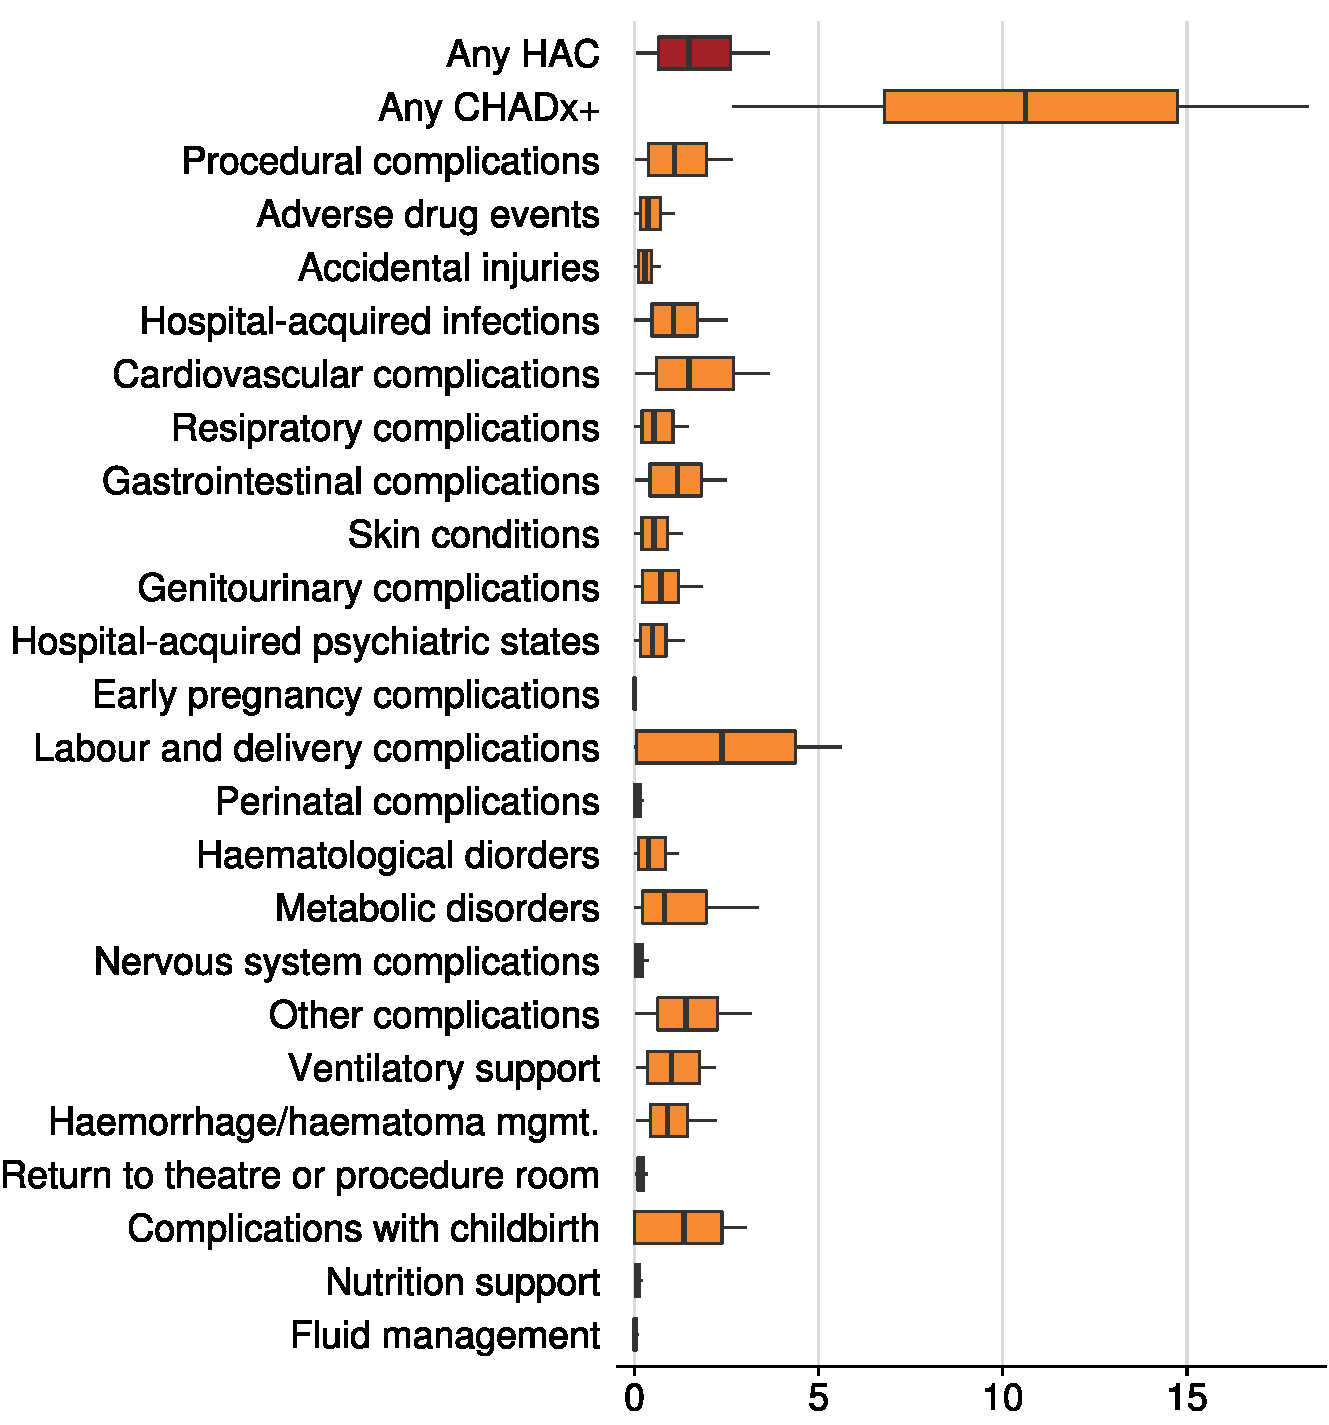
\includegraphics{atlas/boxplot.pdf}
\noteswithsource{As is typical of boxplots, the central line marks the median, the shaded box extends across the interquartile range, and the whiskers of each plot extend out to the 10th and 90th quantiles. This figure is based on raw, not risk-adjusted, hospital complication rates.}%
{Grattan analysis of the 2012-15 National Hospital Morbidity Dataset}
\end{figure}

All of this variation matters, because it represents opportunities to reduce discomfort and harm to patients.
As the following chapter shows, the key opportunities to improve the safety of care are different across hospitals.
Accordingly, safety improvement priorities should be tailored for each hospital, rather than set uniformly across the sector.

More ambitious safety improvement targets would encourage each hospital to focus on the areas where they have the greatest scope to improve.
More granular performance metrics would help them do so.

\subsubsection{Common events are better suited to performance monitoring}\label{subsubsec:common-events-are-better-suited-to-performance-monitoring}

When safety priorities are defined narrowly, we end up monitoring events that are rare.
This data won't necessarily be useful to a hospital that is trying to evaluate and refine its safety improvement initiatives.

It's necessary to monitor rare events over a longer period in order to isolate the trend in the data from the statistical noise.
By the time you have enough information to pin-point a hospital's relative performance, the circumstances surrounding the result may be a distant memory.
It's possible to measure a hospital's performance with greater precision if the performance metric is based on a more common event.
More common events -- such as any complication in overnight patients -- can also be validly used in smaller hospitals and smaller specialties.

\Vref{fig:there-is-scope-to-improve-almost-all-complications} also shows there is considerably more variation in the rate of all complications across hospitals than in HACs rates.%
	\footnote{Based on the interquartile ranges (\ie~the difference between the top and bottom 25 per cent for the two measures).}
As a consequence, over a given time period rates for all complications identify hospitals' relative performance with greater precision than the incidence of HACs.
	
Where a given level of precision is required, it's also possible to report rates for all complications more frequently.
Consequently, it's easier to observe changes in each hospital's safety through its overall incidence of complications.
This issue is discussed in more depth, including the implications for small hospitals, in the Methodological Supplement to this report.

\subsubsection{Easy targets are lazy targets}\label{subsubsec:easy-targets-are-lazy-targets}

Setting a target involves balancing the costs of getting to the target with the benefits that will be achieved.
We know that it is easier to improve the performance of the worst hospitals than in the average hospital,%
	\footcites{Ivers_2012}{Mendelson_2017}
but that does not mean our ambition should be so limited.

Vastly more patients are treated in the middle-performing 80 per cent of hospitals than in the worst 10 per cent of hospitals.
So improving the performance of that middle group will benefit vast numbers of patients. 
Hospitals in the middle band should not be allowed to wallow in complacency, when other hospitals, faced with the same budget constraints, are doing so much better.

Ambitious targets should therefore be set: the aim should be to get all hospitals up to the level of the best 10 per cent, rather than focussing only on improving care in the worst-performing hospitals.

The following chapter shows that, with granular performance metrics, Australia can move beyond artificially narrow lists and start identifying where hospitals' specific safety improvement opportunities lie.












\chapter{Data can inform hospitals about their specific strengths and weaknesses}\label{chap:data-can-inform-hospitals-about-their-specific-strengths-and-weaknesses}

\Chapref{chap:the-harm-done} argued that Australia should study the full range of patient outcomes, particularly the better-than-expected results, rather than only the rare catastrophes.

\Chapref{chap:australia-needs-to-set-more-ambitious-hospital-safety-targets} showed that the narrow view of `harm' to patients in Australian hospitals matters because it drastically underestimates the scope for improving hospital safety and may create incentives to ignore important opportunities.

A comprehensive view of complications is needed.
The substantial variation found in the general quality of hospital care means that substantial data-driven quality improvement is within reach.

This chapter demonstrates how that can be done.
It interrogates the routine data to answer three questions: What are specific hospitals' strengths and weaknesses? Who excels at different aspects of care? And what does this mean for specific patients, and their healthcare decisions?

We've used anonymised routine data (that is, it does not identify particular hospitals or patients) to quantify how much variation there is in the safety of Australia's hospitals.
The Australian Institute of Health and Welfare dataset we use includes data from all admissions to Australia's public and private hospitals between July 2012 and June 2015.
\Vref{box:a-patient-story} gives an example of how much information this dataset contains about individual patients' hospital stays.

By comparing risk-adjusted complication rates across hospitals, we identify the extent to which safety could be improved overall, and what this means for specific institutions and their patients.

The fact that there are big differences between hospitals highlights another important policy issue -- hospitals and their clinicians need to have access to this information so they can analyse their performance and identify opportunities for improvement.
We discuss this issue in \Chapref{chap:we-need-to-share-data-openly}.

\begin{bigbox*}{Belinda's story}{box:a-patient-story}

Australia's routine hospital datasets contain rich information about patients' hospital stays.
For example, \emph{here is Belinda's story}:

Belinda, a 55-year-old woman from Dromana in Victoria, was recommended to have a knee replacement.%
	\footnote{Not her real name, age or suburb.}
She is a smoker, but presented with no comorbidities.

The procedure went according to plan, except she bled heavily after the operation.
Belinda's rehab went well until she contracted a bad strain of pneumonia that appeared to be making its way around the hospital.

What should have been a five-day admission extended to eight, and Belinda had to spend an extra week in bed at home recovering from pneumonia.
This hindered her rehabilitation efforts after the knee replacement and delayed her return to work.

\vfill\null\eject
\textbf{And here is what we see in the data set:}\\
\begin{tabularx}{1\linewidth}{lcX}
\multicolumn{3}{>{\bfseries}l}{Principal diagnosis:} \\
& M171 & Primary gonarthrosis \\[1\baselineskip]
\multicolumn{3}{>{\bfseries}l}{Additional diagnosis present on admission:} \\
& F171 & Harmful use of tobacco \\[1\baselineskip]
\multicolumn{3}{>{\bfseries}l}{Principal procedure:} \\
& 4951800 & Total arthroplasty of the knee, unilateral \\[1\baselineskip]
\multicolumn{3}{>{\bfseries}p{\linewidth}}{Additional diagnoses which occurred during the course of the admission:} \\
& J189 & Pneumonia\\
& D649 & Anaemia\\
& D686 & Thrombophilia (with presence of the lupus anticoagulant)\\
& J440 & Chronic obstructive pulmonary disease (with acute exacerbation)\\
& R090 & Asphyxia
\end{tabularx}\par
\end{bigbox*}

Hospitals and states differ in their coding practices -- an issue discussed in the Methodological Supplement to this report.
In particular, the use of the indicator of whether a diagnosis occurred after admission -- our measure of complications -- varies across states.
These differences make it difficult to validly compare hospital performance across states, and so the analysis in this report focuses on within-state variation.%
	\footnote{All figures that relate to the scope to improve complication rates are net of differences in the mean complication rate across states.}

	There are weaknesses in the existing data -- as described in \citetitle{DuckettEtAl-2017-Strengthening-safety-statistics}.\footcite{DuckettEtAl-2017-Strengthening-safety-statistics}
But this same dataset is used for determining funding flows from the Commonwealth Government to the states, and for determining the apparent safety-related penalties applied by the Commonwealth Government.
This suggests that the dataset is good enough to be used more extensively for measuring safety of care.

Over time, coding can be expected to improve -- especially as the routine data improves with use and as recommendations in our previous report on improving data quality are implemented.

In the longer term, the quality of recording and coding will also improve with the advent of an electronic health record and associated decision-support systems which will automate many of the existing manual data recording and coding tasks.%
	\footcites{Stanfill_2010}{Scheurwegs_2017}{berndorfer2017automated}

\section{Fair comparisons of complication rates across hospitals are now possible}\label{sec:fair-comparisons-of-complications-rates-across-hospitals-are-now-possible}

Of course, complications are easier to avoid in patients who are in better health.
This means fair comparisons can only be made across hospitals if the complication rates are adjusted for patients' `risk profiles'.%
	\footnote{Or are presented in terms of like groups -- a process known as risk stratification.
	We use risk adjustment in this report.}

Risk adjustment has been employed in medical research since the 19\textsuperscript{th} century.%
	\footcites{iezzoni1996apples}{iezzoni1997risks}
However, there is continuing debate about what constitutes adequate risk adjustment, and whether data held in the routine data sets is adequate for the task.%
	\footcite{alexander2017risks}

Australia's routine hospital data details patients' diagnoses, comorbidities and procedures, as well as their age, sex and socio-economic status.%
	\footnote{Even better risk adjustment could be possible if more clinical data, such as pathology test results, were incorporated into the routine data set, as Grattan Institute has previously shown (\textcite{DuckettEtAl-2015-Questionable-care}).}
In this report we use this information to conduct very extensive risk-adjustment.
In our analyses, we adjust for the impact of patient characteristics such as age, sex, the severity of diagnoses and whether the patient has any comorbidities.
Our model allows the risk associated with each of these factors to vary by Diagnosis Related Group.%
	\footnote{Whether factors related to health inequalities should be controlled for is debatable: these factors contribute to patients' risk profiles in ways that we hope clinicians can overcome.
	To control for these factors is to excuse different outcomes.
	We take a moderate approach and control for socio-economic status but not other factors such as indigeneity and cultural and linguistic diversity.
	See the Methodological Supplement for a full discussion of our approach.}
For example, we account for whether a patient has other health issues such as a respiratory condition, and the contribution of these patient factors to our estimates of their risk of a complication are different for patients with different primary diagnoses.%
	\footnote{The risk adjustment underpinning the following results is substantially more detailed than the methodology proposed by \textcite{IHPA-2017-Risk-adj-model-tech-specs} for introducing risk-adjusted financial penalties for HACs and the level of risk-adjustment that is considered appropriate in many academic publications (for example, \textcite{zhang2013patient}).
	Please see this report's Methodological Supplement for further details.}

After these adjustments have been made, the scope for better outcomes can be estimated as the difference between each hospital's rate of complications and the lowest risk-adjusted rate observed at any hospital.

\Vref{fig:headline-complication-rates-dont-reveal-whether-hospital-perf-better-than-exp}  illustrates the importance of this risk-adjustment process.
A hospital can have a higher rate of complications than its peers, but still have a lower rate than expected given the risk profile of its patients.
For example, hospital 558 has a higher complication rate than hospital 302.
But hospital 558's rate is lower than expected given the sort of patients it treats, whereas hospital 302's rate is higher than expected given the sort of patients it treats.

\section{Routine data can illuminate paths to safer care}\label{sec:routine-data-can-illuminate-paths-to-safer-care}

Comparisons of risk-adjusted outcomes across hospitals can provide useful information about hospitals' relative strengths and weaknesses, the nature of the harm that particular patients are most susceptible to, and which hospitals are likely to be safest for patients with particular characteristics.

To illustrate these trends, we use three case studies: patients admitted for cardiology issues who do not have a procedure, patients admitted for knee replacement, and patients admitted for bariatric surgery.
Only multiday admissions are included.

\Vref{fig:3-2-hosp-perf-explains-8-10pc-var-patient-outcomes} shows that hospital performance explains about 8-10 per cent of the variation in a patient's risk of a complication.

\doublecolumnfigure{
\caption{Headline complication rates don't reveal whether a hospital is performing better than expected}\label{fig:headline-complication-rates-dont-reveal-whether-hospital-perf-better-than-exp}
\units{Share of admissions involving at least one complication (actual rate) relative to expected rate given the risk profile of hospital's patients, multiday cardiology admissions that do not involve a major procedure, per cent}
\includegraphics[page=10]{atlas/comps_charts.pdf}
\source{Grattan analysis of the 2012-15 National Hospital Morbidity Dataset}
}{
\caption{Hospital performance explains 8-10 per cent of the variation in patient outcomes}\label{fig:3-2-hosp-perf-explains-8-10pc-var-patient-outcomes}
\units{Proportion of variation in complication rates explained by hospital performance and patient risk, per cent}
\includegraphics[page=11]{atlas/comps_charts.pdf}
\source{Grattan analysis of the 2012-15 National Hospital Morbidity Dataset.}
}


In the following sections, we use these three case studies to show what can be learned from Australia's existing routine data.

Of course, the routine data is not the only source of information on hospital safety.
Useful and complementary information about bariatric surgery and knee replacements are captured by clinical quality registries.%
	\footnote{For more on how to improve the clinical quality registries, see \citetitle{DuckettEtAl-2017-Strengthening-safety-statistics}.}
Our analyses of routine data illustrate what's currently possible to know about all hospital admissions, regardless of whether any registry data is available.

\subsection{Data can illuminate where the biggest opportunities for safety improvement lie}\label{subsec:data-can-illuminate-where-the-biggest-opportunities-for-safety-improvement-lie}

Our analysis of cardiology admissions indicates that if all hospitals were to become as safe for cardiology patients as the safest 10 per cent, 12,000 fewer cardiology patients would experience complications during their admission.
The size of this opportunity varies by institution.

\Vref{fig:hospital-safety-varies-significantly-within-states-and-sectors} shows there are safer and less safe hospitals in every state, and in the private sector.%
	\footnote{It is not possible to draw comparisons across states from \Cref{fig:hospital-safety-varies-significantly-within-states-and-sectors}.
	We have standardised for differences in the average complication rate by state, to take account of state-based differences in coding practices.}
Each dot represents how much greater the risk of a complication is for patients at that particular hospital, relative to the risk they would face at the safest 10 per cent of hospitals in that state or group.

\begin{figure}
\caption{Hospital safety varies significantly within states, and within sectors}\label{fig:hospital-safety-varies-significantly-within-states-and-sectors}
\units{Excess risk of a complication relative to safest 10 per cent of hospitals in that state or group, multiday cardiology admissions that do not involve a major procedure, by hospital, per cent}
\includegraphics[page=14]{atlas/comps_charts.pdf}
\noteswithsource{Excludes small hospitals that were grouped together for the purposes of risk adjustment}{Grattan analysis of the 2012-15 National Hospital Morbidity Dataset}
\end{figure}

Some hospitals are substantially less safe for cardiology patients than others.
\Cref{fig:hospital-safety-varies-significantly-within-states-and-sectors} shows that a patient with an average risk profile in New South Wales faces a 38 per cent higher risk of a complication if they attend the least safe hospital, relative to the risk they'd face at the safest New South Wales hospitals.

\begin{figure}
\caption{The greatest opportunity to make Australian hospitals safer is to move average hospitals closer to excellent hospitals}\label{fig:move-avg-hospitals-closer-to-excellent-ones}
\units{Excess risk of a complication relative to safest hospital for multiday cardiology admissions that do not involve a major procedure, by performance category}
\includegraphics[page=17]{atlas/comps_charts.pdf}
\noteswithsource{By definition, there is no reduction in admissions with complications at hospitals in the best decile of performance if they continue to perform at that level}{Grattan analysis of the 2012-15 National Hospital Morbidity dataset}
\end{figure}

However, this doesn't mean that efforts to improve the safety of cardiology care should be targeted exclusively at those outlier hospitals.
\Vref{fig:move-avg-hospitals-closer-to-excellent-ones} shows that there is also a substantial difference between the excess risk at average-performing hospitals and the best decile.
Most patients are treated in these average hospitals.
If the general safety of hospital care could be improved to the best decile level, 12,000 more admissions could be complication-free every year.
We should be helping every hospital learn from the best.

\subsection{Data can show hospitals where improvement is needed}\label{subsec:data-can-show-hospitals-where-improvement-is-needed}

Hospitals would be better able to improve the safety of their care if they had two sets of information about the incidence of complications in their hospital.

Firstly, hospitals need to know where they have the greatest scope to improve.
\Vref{fig:safety-of-hospitals-care-varies-by-specialty} shows that the safety of hospitals' care varies by specialty.

\begin{figure}
\caption{The safety of a hospital's care can vary by specialty}\label{fig:safety-of-hospitals-care-varies-by-specialty}
\units{Excess risk of a complication relative to safest 10 per cent of hospitals, by admission type, multiday admissions only, per cent}
\includegraphics[page=12]{atlas/comps_charts.pdf}
\source{Grattan analysis of the 2012-15 National Hospital Morbidity Dataset}
\end{figure}

Hospital 803 is in the top 10 per cent of hospitals for medical cardiology and just outside the top 10 per cent for all multiday non-obstetric admissions, but its knee replacement patients face a risk of a complication more than 13 per cent higher than such patients at hospitals which excel in this speciality.
Hospital 105, on the other hand, is a relatively poor performer: its patients generally face at least a 10 per cent higher chance of a complication than patients at the safest hospitals.
However, its knee replacement patients are safer than those at hospital 803.

Hospitals do tend to be good in a number of areas or less good in a number of areas.
But data can be used to identify ``hot spots'' so that the scarce resources devoted to improving care can then be allocated to them.%
	\footnote{Accepting also that institution-wide strategies, such as improved handover, may influence the occurrence of a range of complications and in many types of patients.}
At the moment this hospital-specific information is retained by health departments.
If it were made available to the hospitals, they would be better equipped to improve the safety of their care.

The second set of information that could help hospitals improve the safety of their care is detailed data on the types of complications which are most common among patients of different types.

Providing such detailed information about hospitals' relative performance across different specialties, and the complications that affect particular types of patients, would enable hospitals to target their safety improvement efforts where they have the greatest scope to improve.

\subsection{Data can help patients make better decisions about their health care}\label{subsec:data-can-help-patients-make-better-decisions-about-their-health-care}

Patients should know what outcomes to expect, and what complications they may face.
Such information may affect their care choices and the focus of their pre-operative preparation and post-operative rehabilitation.

Existing data can sometimes provide answers to common questions such as: `Which hospitals achieve the best outcomes for people like me?'

Just as different hospitals have different patterns of complications, so too some hospitals are better than others at treating patients in different age groups.
\Vref{fig:3-7-safe-choice-varies-by-age} shows estimates of excess risk for three hospitals that perform knee replacements.

\begin{figure}
\caption{The safest choice can vary for patients of different ages}\label{fig:3-7-safe-choice-varies-by-age}
\units{Excess risk of a complication relative to safest hospital for that age group, knee replacement admissions, per cent}
\includegraphics[page=19]{atlas/comps_charts.pdf}
\source{Grattan analysis of the 2012-15 National Hospital Morbidity Dataset}
\end{figure}

It shows that Hospital A is a uniformly good hospital to go to for a knee replacement, and Hospital C is uniformly bad.
At Hospital B, patients over 75 face twice the excess risk of a complication compared to similar patients at Hospital A, but their excess risk for other patients is similar to the performance in Hospital A.

More multidisciplinary care and specialised attention to rehabilitation may be reasons why Hospital A is able to reduce the occurrence of complications in the very old.
The value of such data for identifying complications for the elderly is evident.

\section{Current approaches to measuring safety are out of date}\label{sec:current-approaches-to-measuring-safety-are-out-of-date}

The insights that can be extracted from our existing data sources using approaches that have been available for ten years raises the question: Why are these analyses not performed regularly in Australia?

The answer may relate to implicit safety beliefs: that harm is uncommon and extreme, and that someone is to be blamed.
This mindset leads to clinicians being anxious about data being shared and analysed.
Yet this chapter has demonstrated that complications are common, rather than rare and extreme events.
This finding justifies a totally different approach to transparency.

This report particularly focuses on reporting comparative hospital performance, an area where Australia is a relative laggard given international recognition that `Robust comparison of performance with peers is fundamental to securing improvement'.%
	\footcite{OECD-2017-Health-at-a-glance}

The next chapter shows how increased transparency about the data could transform Australia's approach to safety improvement.
















\chapter{We need to share data openly}\label{chap:we-need-to-share-data-openly}

Australia needs a comprehensive approach to variations in the outcomes of hospital care and the occurrence of complications.
While once patient safety efforts were focused on serious incidents and deaths judged to be preventable, we now know that everyday instances of suboptimal care cause substantial harm.

This report's analysis of routine data shows how much improvement can be made.
This final chapter details the changes required to close the gap we have identified between the safety of care that is given in Australian hospitals and that which could be given.
It makes recommendations designed to ensure more hospitals deliver care that is as good as the top 10 per cent of hospitals.

The recommendations in this chapter complement those in Grattan Institute's previous report, \citetitle{DuckettEtAl-2017-Strengthening-safety-statistics}.
That report looked at improving the data sources we use to monitor safety, including the need to ensure the quality of coding remains strong so that routine data can be used confidently for both payment and safety monitoring.%
	\footcite{DuckettEtAl-2017-Strengthening-safety-statistics}

Hospitals' own internal efforts to improve safety of care requires attributable and specific information.%
	\footcite{Levesquee014825}
Grattan's next report will look at strengthening the external motivators of hospital activity, such as accreditation processes.

All the recommendations in this report are about better using the existing data which is collected from hospitals -- publishing it, and providing it to those best placed to use it.
The recommendations do not require collection of any additional data, and so implementation costs are small.
The benefits of implementation, however, are large in terms of improving the safety of patient care.

The recommendations are also about redirecting existing effort -- away from dramatic complications that happen rarely, toward more `ordinary' complications that happen often.
Because so many more people would benefit, this would be a better use of the time that clinicians already spend on addressing safety issues in their hospitals.

\section{Governance mechanisms need to assure safety}\label{sec:governance-mechanisms-need-to-assure-safety}

Accreditation, governance and pricing systems play an important role in ensuring minimum safety standards are met in Australian hospitals.
They affect the priorities of and constraints on hospital management teams.
Safety performance information should be central to these systems.%
	\footcite{Levesquee014825}

Hospital management is an extremely difficult task.
Hospitals are big and complex organisations, expected to deliver care that is accessible and cost-effective as well as of high quality.
This `triple aim' means that hospitals' efforts to improve the quality and safety of care must be managed alongside efforts to improve access and to constrain costs.%
	\footnote{The term `triple aim' was coined by the United States Institute for Healthcare Improvement and referred to improving the experience of care, improving the health of populations, and reducing per capita costs of health care; see \textcite{Berwick_2008}.}
Time and resources invested into quality improvement is not available to improve waiting times.

The trade-offs between these objectives are not pre-determined -- they are the consequence of policy.
Accreditation standards define minimum safety and quality processes, the hospital pricing regime defines the financial constraints within which this must be delivered, and health departments set access targets.
Governance activities -- through boards and health departments -- routinely monitor progress on all these measures.

When these systems work well, they highlight meaningful safety requirements, effectively support management to deliver them, and minimise the tensions between quality and cost objectives.
But when they don't, it can be difficult for management to improve safety.
Tensions with financial and access objectives can obscure the business cases for safety initiatives.%
	\footnote{A future Grattan Institute report will deal more explicitly with financial incentives and business cases.}

The role of a regulator should be to eliminate unwarranted variation in performance.%
	\footcite{Hollnagel-2014-Safety-Management}
For the hospital system -- both public and private -- the regulator is the state government, through its health department.
States should address the wide variation in rates of complications highlighted in this report.
They should rise to the challenge of helping hospitals and clinicians to drive down rates of all complications, not just focus on the smaller subset of complications which have been labelled as `preventable'.

The reforms needed to ensure Australia's hospital accreditation, governance and pricing systems all support reliably safer care are beyond the scope of this report, and will receive fuller attention in our next report.
But governance changes need to be accompanied by quality improvement work -- which requires providing data to clinicians and patients, setting targets, and supporting the subsequent improvement endeavours.

\section{Measure and report on all complications -- not a subset}\label{sec:measure-and-report-on-all-complications-not-a-subset}

Clinicians and managers are hungry for more data.%
	\footcites{Jorm-2017-Clinical-engagement}{Duckett-Review-2016-Quality-assurance-in-Vic}
Currently 92 public and private health service organisations across Australia and New Zealand are members of a private benchmarking group called The Health Roundtable.%
	\footnote{See: \textcolor{blue}{\url{https://www.healthroundtable.org/}}.}
They pay their fees and submit their data because participation provides comparative information for improvement that they cannot obtain otherwise.

Comparative data for improvement should systematically identify all opportunities to reduce harm.
Narrow `indicator' sets are inconsistent with new theoretical thinking on how to make systems safer.
They also distort priorities because, as shown in \Vref{fig:safety-of-hospitals-care-varies-by-specialty}, within hospitals some clinical specialties and care teams do better than others.

There is another issue with indicator sets, as illustrated by the ossification of the Australian sentinel event lists, discussed in \Cref{sec:australia-has-three-key-measures-of-unsafe-care}.
It was borrowed from a US list that has since developed considerably.
Unfortunately, the Australian sentinel events list did not evolve and a revision is only now awaiting approval, and there is clearly the risk that HACs will meet the same fate.%
	\footnote{Although this risk is mitigated by revision of the HACs list being on the work program of the Australian Commission on Safety and Quality in Health Care.}

Measuring all complications ensures a dynamic approach to improving safety.
As the complication profile of patients and hospitals changes, new targets for improvement can be set.

\subsection{Reporting to hospitals }\label{subsec:reporting-to-hospitals}

The data currently kept within state health departments should be made available to all relevant parties: hospitals, clinicians, patients and the wider public.
This information should be provided to hospitals in a form that can be analysed and then used to help clinicians improve the safety of care.
It should also be provided to the public, so people can hold hospital managers accountable.

State health departments have the capacity to risk-adjust and report comparative data.
They should give hospitals regular, specific updates of how their performance compares to their peers'.
\Vref{fig:heatmap} provides an example of how this could be done.
It shows the quintile of a given hospital's risk-adjusted performance overall, by each of the Major CHADx and CHAPx classes, and by each of the Minor CHADx+ classes.


\begin{figure*}
\newcommand{\cellYellow}{\cellcolor{Color1}}
\newcommand{\cellOrange}{\cellcolor{Color3}}
\newcommand{\cellRed}{\cellcolor{Color5}}
\newcommand{\celltheGrey}{\cellcolor{theGrey!80}}

\newcommand{\qa}{\cellcolor{Color2}}
\newcommand{\qb}{\cellcolor{Color3}}
\newcommand{\qc}{\cellcolor{Color4}}
\newcommand{\qd}{\cellcolor{Color5}}
\newcommand{\qe}{\cellcolor{Color6}}
\newcommand{\qf}{\cellcolor{theGrey!75}}
\newcommand{\qg}{\cellcolor{theGrey!25}}

\newcolumntype{C}{>{\centering\arraybackslash}p{10pt}}

\caption{Hospitals should regularly receive heat maps of their relative performance}\label{fig:heatmap}
\begin{tabular}{@{}rlc*{23}{C}}
\toprule
&   &\multicolumn{24}{c}{Minor CHADx or CHAPx class} \\
\cmidrule{3-26}          
\multicolumn{2}{l}{\textbf{Major CHADx class}}  & Maj.\space & 1   & 2   & 3   & 4   & 5   & 6   & 7   & 8   & 9   & 10  & 11  & 12  & 13  & 14  & 15  & 16  & 17  & 18  & 19  & 20  & 21  & 22  & 23  \\
\midrule
1  & Post-procedural complications  & \qd & \qd & \qe & \qa & \qd & \qd & \qe & \qd & \qc & \qd & \qd & \qc & \qd & \qd & \qe & \qe & \qa & \qa & \qd & \qd & \qd & \qd & \qd & \qb \\
2  & Adverse drug events            & \qd & \qf & \qf & \qf & \qf & \qf & \qf & \qf & \qf & \qf & \qf & \qf & \qf & \qf & \qd & \qd & \qd & \qd & \qd & \qg & \qg & \qg & \qg & \qg \\
3  & Accidental injuries            & \qc & \qf & \qf & \qf & \qf & \qe & \qa & \qc & \qg & \qg & \qg & \qg & \qg & \qg & \qg & \qg & \qg & \qg & \qg & \qg & \qg & \qg & \qg & \qg \\
4  & Specific infections            & \qc & \qd & \qd & \qd & \qe & \qb & \qc & \qd & \qc & \qc & \qd & \qd & \qc & \qc & \qe & \qd & \qc & \qb & \qe & \qe & \qc & \qg & \qg & \qg \\
5  & Cardiovascular complications   & \qc & \qd & \qd & \qd & \qd & \qe & \qd & \qd & \qd & \qc & \qd & \qd & \qe & \qe & \qg & \qg & \qg & \qg & \qg & \qg & \qg & \qg & \qg & \qg \\
6  & Respiratory complications      & \qc & \qd & \qd & \qc & \qd & \qd & \qc & \qe & \qg & \qg & \qg & \qg & \qg & \qg & \qg & \qg & \qg & \qg & \qg & \qg & \qg & \qg & \qg & \qg \\
7  & Gastrointestinal complications & \qc & \qd & \qd & \qd & \qb & \qc & \qd & \qg & \qg & \qg & \qg & \qg & \qg & \qg & \qg & \qg & \qg & \qg & \qg & \qg & \qg & \qg & \qg & \qg \\
8  & Skin conditions                & \qc & \qc & \qd & \qe & \qc & \qg & \qg & \qg & \qg & \qg & \qg & \qg & \qg & \qg & \qg & \qg & \qg & \qg & \qg & \qg & \qg & \qg & \qg & \qg \\
9  & Genitourinary conditions       & \qd & \qd & \qd & \qc & \qd & \qg & \qg & \qg & \qg & \qg & \qg & \qg & \qg & \qg & \qg & \qg & \qg & \qg & \qg & \qg & \qg & \qg & \qg & \qg \\
10 & Hospital-acquired
                 psychiatric states & \qc & \qb & \qa & \qb & \qd & \qd & \qb & \qc & \qg & \qg & \qg & \qg & \qg & \qg & \qg & \qg & \qg & \qg & \qg & \qg & \qg & \qg & \qg & \qg \\
14 & Haematological disorders      & \qc & \qe & \qc & \qd & \qb & \qg & \qg & \qg & \qg & \qg & \qg & \qg & \qg & \qg & \qg & \qg & \qg & \qg & \qg & \qg & \qg & \qg & \qg & \qg \\
15 & Metabolic disorders           & \qd & \qd & \qd & \qd & \qd & \qd & \qd & \qg & \qg & \qg & \qg & \qg & \qg & \qg & \qg & \qg & \qg & \qg & \qg & \qg & \qg & \qg & \qg & \qg \\
16 & Nervous-system complications  & \qc & \qd & \qc & \qd & \qg & \qg & \qg & \qg & \qg & \qg & \qg & \qg & \qg & \qg & \qg & \qg & \qg & \qg & \qg & \qg & \qg & \qg & \qg & \qg \\
17 & Other complications           & \qb & \qd & \qa & \qb & \qd & \qc & \qc & \qd & \qb & \qb & \qc & \qc & \qg & \qg & \qg & \qg & \qg & \qg & \qg & \qg & \qg & \qg & \qg & \qg \\
\phantom{.}        & \\[-0.5\baselineskip]
\multicolumn{3}{l}{\textbf{Major CHAPx class}} \\
\midrule
1 & Ventilatory support              & \qd & \qe & \qd & \qg & \qg & \qg & \qg & \qg & \qg & \qg & \qg & \qg & \qg & \qg & \qg & \qg & \qg & \qg & \qg & \qg & \qg & \qg & \qg & \qg \\
2 & Haemorrhage/haematoma mgmt & \qd & \qe & \qd & \qg & \qg & \qg & \qg & \qg & \qg & \qg & \qg & \qg & \qg & \qg & \qg & \qg & \qg & \qg & \qg & \qg & \qg & \qg & \qg & \qg \\
3 & Return to theatre/proc.\ room & \qd & \qe & \qe & \qd & \qe & \qd & \qg & \qg & \qg & \qg & \qg & \qg & \qg & \qg & \qg & \qg & \qg & \qg & \qg & \qg & \qg & \qg & \qg & \qg \\
5 & Nutrition support                & \qe & \qe & \qg & \qg & \qg & \qg & \qg & \qg & \qg & \qg & \qg & \qg & \qg & \qg & \qg & \qg & \qg & \qg & \qg & \qg & \qg & \qg & \qg & \qg \\
5 & Fluid management                 & \qa & \qa & \qg & \qg & \qg & \qg & \qg & \qg & \qg & \qg & \qg & \qg & \qg & \qg & \qg & \qg & \qg & \qg & \qg & \qg & \qg & \qg & \qg & \qg \\
\bottomrule
\phantom{.} \\
  &                                & & \multicolumn{3}{r}{Best quintile} & \qa & & \qb & & \qc & & \qd & & \qe & \multicolumn{4}{l}{Worst quintile} & \\
\null & \\[-0.5\baselineskip]
  & \multicolumn{5}{r}{Data not available to Grattan} & \qf &  \\
  & \null
\end{tabular}
\noteswithsource{Minor CHADx+ classes are particular conditions that are classified within the major CHADx or CHAPx category}{Grattan analysis of the 2012-15 National Hospital Morbidity Dataset}
\end{figure*}


% \begin{figure}
% \caption{Hospitals should regularly receive heat maps of their relative performance}\label{fig:heatmap}
% \units{Heat map of Hospital 1's performance quintiles by CHADx+ subclass}
% \includegraphics[page=20]{atlas/comps_charts.pdf}
% \noteswithsource{CHADx+ subclasses are particular conditions that are classified within the major CHADx or CHAPx category}{Grattan analysis of the 2012-15 National Hospital Morbidity Dataset}
% \end{figure}

Providing Australian hospitals with `heat maps' like this would not be difficult.
The Methodological Supplement to this report outlines the analytic approaches underpinning \Cref{fig:heatmap}, and indicates how large a hospital needs to be for the metric to be meaningful.

The newest edition of the Australian Commission on Safety and Quality in Health Care's National Standards includes a specific requirement under Clinical Governance for hospitals to analyse how clinical practice varies, and to communicate this to their workforce.
This is a step forward, but the exercise will be futile unless states provide hospitals with comparative information.

The National Standard on Clinical Governance requires hospitals to focus on variation.

Under Standard~1.28, Variation in clinical practice and health outcomes, the health service organisation has systems to:

\begin{enumerate}
	\renewcommand{\labelenumi}{\bfseries\color{Orange}\alph{enumi}. }
	\item Monitor variation in practice against expected health outcomes
	\item Provide feedback to clinicians on variation in practice and health outcomes
	\item Review performance against external measures
	\item Support clinicians to take part in clinical review of their practice
	\item Use information on unwarranted clinical variation to inform improvements in safety and quality systems
	\item Record the risks identified from unwarranted clinical variation in the risk management system
\end{enumerate}

\subsection{Reporting to clinicians}\label{subsec:reporting-to-clinicians}

Australia has generally relied heavily on grassroots innovation for safety improvement.
Individual clinicians and hospitals have developed their own internal monitoring strategies, and a plethora of small initiatives are underway in most hospitals.%
	\footnote{Indeed, Victorian clinicians and managers recently complained about an exhausting excess: \textcite{Jorm-2017-Clinical-engagement}.}

Clinical and managerial staff strive for improvement, but are not supported adequately by data that helps them achieve it.%
	\footcite{leggat2017qualitative}
Unfortunately, time-limited projects unsupported by data do not create sustainable change.
Few quality improvement initiatives (including internationally) have been rigorously evaluated.%
	\footcites{Nicolay_2011}{Jones_2016}{Dixon-Woods-Martin-2016-Does-QI-improve-quality}{dixonwoods2016patient}{walsh2014undetermined}
Without continuous provision of robust data, there is `action without knowledge' -- that is, activities that may add to staff workload without improving patient care.%
	\footcites{pronovost2017creating}{kreindler2016what}{Hoog-2016-Quality-improvement-large-orgs}

Our analysis in \citetitle{DuckettEtAl-2017-Strengthening-safety-statistics} of all available safety and quality data sources revealed limitations can be fixed.%
	\footcite{DuckettEtAl-2017-Strengthening-safety-statistics}
Inadequate access to data is making it harder for clinicians to improve safety than it should be.

More data should be placed in the hands of clinical teams.
Considerable information about their practice is collected; they should be given timely access to it. With the advent of electronic health records in hospitals, this could be near real time (see \Vref{box:developing-real-time-safety-data}).

Data at the level of detail in the heat map in \Vref{fig:heatmap} should be provided to clinical teams to help target efforts to specific groups of clinicians and to specific conditions.
Reporting should also describe excess complications in each specialty, and it should provide detail on the outcomes (including length of stay, and readmissions) of high-volume conditions and procedures.

In the UK's `Getting it right the first time' program, for example, specialist clinicians in hospitals are presented with all the available data about their patients, including activity and cost as well as outcomes.
This enhances peer and management review of the performance of individual specialists.%
	\footcite{Timmins-2017-Tackling-variations-in-clinical-care}
In Australia, the medical colleges would be ideally placed to lead such reviews.

A focus on all complications would cast the net for identifying improvements much wider -- specialty groups in larger hospitals would be able to focus on their own priorities, unconstrained by whether they are on the HAC list or not.

New South Wales already provides clinicians with access to a dataset which enables them to compare their performance with other similar clinical teams.%
	\footnote{See: \textcolor{blue}{\url{http://www.health.nsw.gov.au/wohp/Documents/mc2-abm-adamato.pdf}}\,.}
All states should follow suit.
But each state does not need to reinvent this wheel.
	The National Benchmarking Portal established by the Independent Hospital Pricing Authority%
		\footnote{See: \textcolor{blue}{\url{https://www.ihpa.gov.au/what-we-do/data-collection/national-benchmarking-portal}}\,.}
currently focuses on cost-benchmarking.
It should be expanded to enable easy comparison of complication rates.

\begin{smallbox}{Developing real-time safety data}{box:developing-real-time-safety-data}

This report uses a large national dataset to demonstrate the opportunity for improvement.
However, as we argued in \citetitle{DuckettEtAl-2017-Strengthening-safety-statistics}, to be useful for improvement, comparative information needs to be timely.%
	\footcite{DuckettEtAl-2017-Strengthening-safety-statistics}
Information about safety reaches its `use-by' date surprisingly quickly.
Real-time data is the new `gold standard'.
Information about recent complications is interesting, but information about unfolding events is riveting, because clinicians can act in response.%
	\footnote{During the consultation phase on this report one commentator highlighted this, saying: `We have been giving really extensive retrospective data to our hospitals for five years now, outlining many opportunities for improvement.
	Yet, as soon as it was real time, an impetus for change was generated that all the retrospective data given to date couldn't generate.
	I don't quite understand why, but it is very real.' A second commentator echoed this: `My early experience with the digital hospital is that we are able to build, in real time, lead indicators which trigger clinician action and intervention in the face of variation, flagging signs of deterioration, poor glycaemic control, \etc.'}
An electronic medical record that provides decision support, and with data collected during care rather than coded \emph{after} discharge, is a basic 21\textsuperscript{st} century tool.
Yet, implementation of these systems in Australia is still embryonic.%
	\footcite{Sullivan_2016}
\end{smallbox}

\CenturyFootnote
\subsection{Reporting to the public}\label{subsec:reporting-to-the-public}

Expectations about public reporting are changing both by governments -- who are actively looking at improving reporting%
	\footnote{A recent decision of Health Ministers supported work on national consistency in reporting, see: \textcolor{blue}{\coagURL}\,.} %
\space\textendash{} and from patients.
States should report hospital outcomes data relevant to patients' care decisions in a way that is readily accessible to patients and GPs.
State reporting about public and private hospitals should be quite detailed -- reporting all complications classified into Minor CHADx+ classes.
An interactive website should be created to enable more specific reporting relevant to patients, such as by age and sex.%
	\footcite{Greenhalgh_2017}

\begin{smallbox}{Reporting by private hospitals}{box:reporting-by-private-hospitals}

A number of private hospital groups, such as Healthscope\footnote{See: \textcolor{blue}{\url{http://www.healthscopehospitals.com.au/quality/my-healthscope/}}.}
	and Ramsay,\footnote{See: \textcolor{blue}{\url{http://www.ramsayhealth.com/Sustainability/Patient-Safety-and-Quality/Latest-Results/}}.}
publicly share their safety and quality measures.
Intending Healthscope and Ramsay patients are able to see a wide range of results for the group, together with details of improvement initiatives underway.
A comparison with `public hospitals' is also provided, but this information is not risk adjusted -- probably because the private chains do not have the information to do so -- and so patients are not able to make comparisons between particular private hospitals or between particular public and private hospitals.%
	\footnote{An alternative approach suggested in the consultation phase on this report is to provide unadjusted data for particular groups (\eg~stratified by age), so that patients have a better understanding of the risks of admissions.}
\end{smallbox}

New South Wales has made a good start, and its example should be followed by other states and extended to include private hospitals.
Private patients pay extra for (among other things) the opportunity to choose their treating doctor and hospital.
Despite some private hospital chains starting to publish performance information themselves (see \Vref{box:reporting-by-private-hospitals}), at present patient choice is poorly informed, because existing data that robustly compares hospitals and doctors is not made available.

We have provided an example of an interactive website and app at: \ShinyAppURL{}. However, we are not permitted to release hospital-specific information and so the website simply provides Australia-wide information. 
States should develop similar websites which would allow patients to compare complication rates between hospitals, taking account of the patient's age and sex, and ideally any other conditions they have -- such as diabetes -- which influence complication rates.
This information -- as we show in our prototype app -- is available now and should be made available to prospective patients.

Private health insurers have an important role here too.
The larger insurers (Medibank and BUPA), and through a cooperative venture (the Australian Health Services Alliance) many smaller insurers, have sufficient information to produce robust measures of hospital performance.
Indeed, Medibank already provides scorecard information to hospitals which includes data on rates of readmissions, complications, and admissions to intensive care units.%
	\footcite{Rankin-2017-Outcome-measurement-in-private-hospital}

Private health insurers should share that same information with their members, to help members make fully informed choices about where they have their elective procedures.

Australians should have access to comprehensive, risk-adjusted, institution-level data for every institution.

Australia's hospital system lags behind international peers in making this transition to greater transparency.
New York State, for instance, commenced public reporting of cardiac surgeons' clinical outcomes 25 years ago.
The US and the UK now provide detailed, publicly reported information on the safety performance of hospitals and some clinicians.%
	\footnote{For example, \textcites{Leapfrog-2016-compare-hospitals}{NHS-2016-Org-patient-safety-reports-Oct-2015-Mar-2016}{behrendt2016mechanisms}{findlay2016consumers}.
The UK's hospital-specific atlas of variation in outcomes demonstrates the specificity with which hospital performance data can be reported back to hospitals (and also publicly shared), see \textcite{NHS-Atlas-series}.}

There are two compelling reasons for Australia to follow suit.
Most fundamentally, it's important in principle that information about variation in the quality of hospitals' care is shared openly with patients and taxpayers.
Secondly, transparent reporting of performance data is an important tool for improving safety.%
	\footnote{There are some risks associated with transparency; the nature, magnitude and mitigation strategies for these risks is discussed in \Chapref{chap:appendix-the-risks-of-transparency-can-be-mitigated}.}

Review of comparative performance of professionals and hospitals has long been seen as `secret squirrel' business, with review of safety incidents to be conducted by consenting adults in private and shielded from scrutiny by legal privilege.%
	\footnote{Through national or state schemes; see, for example: \textcolor{blue}{\url{http://www.health.gov.au/internet/main/publishing.nsf/Content/qps-info}}.}
In this approach, a doctor's or a hospital's right to privacy or commercial interests has been given greater weight than a patient's or the public's right to know about relative performance.

However, the public's expectations about what they ought to know are changing across all areas.
Comparison websites are common in almost every area of consumer choice.
Health care is not immune from this transition.
The culture change from the old-style, secrecy approach will be immense.
It will also require work to ensure that data is presented as clearly as possible so that people can evaluate health risks and benefits.%
	\footnote{The importance of this and methods of supporting both patients and clinicians are discussed in the Grattan Institute's previous report: \textcite{DuckettEtAl-2017-Strengthening-safety-statistics}.}
The change management task for states, hospitals and insurers will also be significant, but it will be worthwhile for patients and for the system as a whole.

\subsubsection{The public has a right to know}\label{subsubsec:the-public-has-a-right-to-know}

The Australian Charter of Healthcare Rights includes the right to receive safe and high-quality care, the right to be informed about services, treatment options and costs in a clear and open way, and the right to participate in decisions about care.%
	\footnote{See: \textcolor{blue}{\url{https://www.safetyandquality.gov.au/national-priorities/charter-of-healthcare-rights/}}. One of the four key themes of the recently released Australian Digital Health Strategy is `Support me in making the right healthcare choices, and provide me with options', see: \textcolor{blue}{\url{https://www.digitalhealth.gov.au/australias-national-digital-health-strategy}}.
	However, the strategic priorities in the strategy will do little to achieve this goal.}
It has been argued that practitioners may have a legal obligation -- as part of their consent procedures -- to disclose information they have about the hospital's rate of complications.%
	\footcite{McWhirter_2017}
Our changing understanding of the nature of most harm caused to patients in hospitals has clear implications for public reporting obligations.

Information about the incidence of extreme harm in specific hospitals is of little relevance to elective patients' choice of hospital or taxpayers' appraisal of their local hospital -- the rarity of these incidents means they are unlikely to reflect hospitals' normal performance.
However, information on the general quality of hospitals' care derived from their relative rates of complications is directly relevant to patients' choices and taxpayers' satisfaction.

Historically, consumers have made limited use of publicly reported comparative performance measures for hospitals.%
	\footnote{\textcite{Greenhalgh_2017}.
	\textcite{Marshall-etal-2000-public-release} found that patients were distrustful of public benchmarking data, and early studies found that leading hospitals don't gain market share after public benchmarking. \textcites{Vladeck_1988}{Weller_2010}{Chassin_2002}{Hibbard_2005}{Jha_2010}.
	But \textcite{mennemeyer1997death} did observe a market response to safety scandals.}
However, this does not mean that they won't use such information in future, or that they are not entitled to it.%
	\footnote{Recent evidence from the US suggests patient engagement with publicly reported performance data is increasing (\textcites{Carman_2016}{Findlay_2016}).
	Other studies are detecting market responses to public benchmarking \textcites{Merle_2009}{Pope_2009}{chen2012public}{Blake_2017}.
	\textcite{Mukamel_2004}
	found that public benchmarking diminishes the influence of experience and price on a patient's choice of surgeon.
	This indicates that patients value information on surgeons' past performance, where such information is available and user-friendly.}
Citizens also require information to fulfil their democratic role of holding government to account.%
	\footcite{Levay_2016}

The patient's GP has an important role here too.
If GPs have better public information -- especially if it is also delivered to their desktop -- their advice to patients about referrals could be more informed and based on the total experience of a specialist or hospital rather than just what the individual GP might have observed from previous referrals.

\subsubsection{Public reporting of hospital safety creates additional incentives for safety improvement}\label{subsubsec:public-reporting-of-hospital-safety-creates-additional-incentives-for-safety-improvement}

When data on hospital performance is fed back to hospitals in a timely fashion, greater safety improvements are achieved.%
	\footcite{Hibbard_2005}
Data makes it easier to identify safety improvement opportunities, and causes management teams and boards to devote more attention to safety.%
	\footcite{Tsai_2015}

Some studies have found that public reporting improves the business case for safety improvements by influencing patients' choice of hospital.%
	\footcite{Chandra_2016}

But the biggest benefit from public reporting appears to be hospitals acting to protect their reputation.%
	\footcites{frlich2007behavioral}{totten2012closing}
Public reporting appears to prompt hospitals to redouble their safety efforts and rethink their hiring strategies.%
	\footcites{Mukamel_2002}{Mukamel_2014}{Chassin_2002}{fung2008systematic}
And sharing data publicly also creates an incentive for state governments to act.
Some hospitals may need more central support.

\subsection{States need to pay attention to issues that are beyond the scope of individual hospitals }\label{subsec:states-need-to-pay-attention-to-issues-that-are-beyond-the-scope-of-individual-hospitals}

Many safety challenges are beyond the capacity of a single institution.
In the absence of support, making individual hospitals solely responsible for improving safety could be as pointless as blaming individuals for system defects.%
	\footcite{dixonwoods2016patient}
The size, staffing and scope of operations of a hospital may all affect its ability to reduce complication rates among patients.
None of these issues are fully within the control of the hospital; all require the involvement of the state.%
	\footnote{For instance a shortage of hospital physiotherapists may be a state-wide or regional problem; solutions may include changes in the relevant employment award.}

State governments also need to build quality improvement capacity across the health system;%
	\footcite{mery2017evaluating}
foster the sharing of knowledge about what is working well; and address broader, whole-system safety issues.
\Vref{subsec:quality-improve} discusses four concepts that are central to supporting improvement efforts.
States also need to reinforce the priority of quality improvement.
It is too easy for states to slip into sending an implicit signal to hospital managers that all that matters are budgets and waiting times.

There are a range of data sources including clinical quality registry data, death audit data, incident reporting and investigation data, patient-reported experience measures, and patient-reported outcome measures that can assist in providing guidance for safety and quality improvement.%
	\footnote{\textcite{DuckettEtAl-2017-Strengthening-safety-statistics}. 
	For an example of an attempt to create a balanced framework that also includes culture and compliance measures, see \textcite{Wakefield_2009}.}
All should be employed when appropriate in the quest to reduce all complications.

The Commonwealth Government should support smaller states and the territories, by providing them with the data to allow them to develop their own approach to national benchmarking (for example, by identifying a relevant cohort of hospitals against which to benchmark), and by publishing national benchmarking data (for example, on what is the best safety performance in a specialty nationally, rather than locally).
Smaller states should also engage with the routine work of the quality improvement bodies of the larger states, for example, the NSW Agency for Clinical Innovation, the Queensland Clinical Excellence Division, and Safer Care Victoria.

\subsection{Supporting quality improvement}\label{subsec:quality-improve}

\subsubsection{Increase clinician engagement}

A pre-condition for serious safety improvement is close working relationships between policy makers, regulators and clinicians.
Australia needs to get better at this. Managers need to give more attention to clinician engagement.
They need to ensure clinicians have sufficient time, resources and skills to pursue safety improvements.
The message should be that safety improvement is not `managers' business' but everyone's business.%
	\footcites{Duckett-Review-2016-Quality-assurance-in-Vic}{Jorm-2017-Clinical-engagement}{Alderwick-etal-2017-Making-case-for-quality-improvement-lessons-for-NHS-boards}

\subsubsection{Foster collaboration}
Cooperative structures such as `clinical networks' or `clinical collaboratives'
create peer accountability and can drive improvement,
although reviews have evaluated their effectiveness as `promising' rather than proven.%
	\footcites{scott2009measurement}{Nelson-2007-Quality-by-design}
Nevertheless, some form of systematic clinical engagement is needed to facilitate sharing of good practice, so that the experience, protocols and procedures used by `positive deviants' becomes part of the routine in all hospitals.
Gone are the days when it was thought that `each organisation should solve their patient safety problems alone'. The more organisations share experiences, data and evidence, the better.

\subsubsection{Design systems that combine accountability and learning}

Any thinking that accountability and learning are incompatible needs to end. 
There should be no dichotomy between information for performance (`for managers') and information for improvement (`for clinicians'). Both require reliable data. (Scotland provides one good model for combining stakeholder engagement, learning and accountability for best results.%
	\footcites{damschroder2014effects}{schang2017complementary})

\subsubsection{Fund programs to reduce complications}
Getting to grips with the full gamut of reducible complications will require new research.
A developmental program should include evidence synthesis, expert review, and research commissioning.
It should study how `positive deviants' deliver safer care, and test the success of applying those lessons in other institutions.
Given the savings which could be generated by reducing complication rates, the Medical Research Future Fund could be directed to develop a program of this kind.
It could be coordinated by the Australian Commission on Safety and Quality in Health Care.

















\chapter{Conclusion}\label{chap:conclusion}

It is unknown how much progress Australia has made on improving patient safety outcomes over the past 20 years.
Internationally, progress is considered to have been disappointing.%
	\footnote{\textcite{Vincent-2016-Safer-Healthcare}. Some studies, for instance in Holland, have demonstrated improvement but there is controversy associated with the validity of longitudinal adverse events studies and their focus on death and error and a call for better, more granular safety metrics. \textcites{Shojania541-Temporal-trends-in-patient-safety-Netherlands}{baines2015effective}{Shojania_2016}.}
For Australia, neither longitudinal adverse event studies nor information about the prevalence of the full range of patient complications has been freely available.

The current incomplete reporting practice, together with a media culture that amplifies sensational events, misleads the public to believe that harm in hospitals is both infrequent and catastrophic.
This obstructs their ability to make informed decisions about their own care.

The lack of sustained attention to reducing all complications is a tragedy, given that some hospitals do so much better than the average.
Australia needs new safety thinking that doesn't normalise harm to hospital patients.
It is time to adopt an epidemiological focus -- examining broad patterns -- and to learn from hospitals and clinicians who achieve low rates of harm.
The policy question is not whether we move to addressing all complications, but when.
The sooner we set more ambitious targets the better.

Priority should be given to seizing opportunities at the local specialty level.
Hospitals and clinicians should be given all the information required to facilitate change.

This report has identified substantial scope to reduce patient harm in Australia, and made recommendations to make our hospitals safer.
Policy makers should now act.

Recommendations:

\begin{itemize}
\item All states and territories establish goals for reducing the overall rate of complications in public and private hospitals.

\item All states and territories give hospitals and clinicians the ability to interrogate the state hospitals data (without individual patients being able to be identified), so they can see how their performance measures up against the best-performing hospitals and clinicians.
All hospitals develop strategies to identify opportunities to improve.

\item All states and territories publish reports on excess complications, by specialty and institution (including private hospitals).

\item Major private health insurers provide their members with comparative information on complication rates.
\end{itemize}





















\appendix
\chapter{The risks of transparency can be mitigated}\label{chap:appendix-the-risks-of-transparency-can-be-mitigated}

Australia has developed a culture of anxiety around the public reporting of hospital activities.
It has manifested as a reluctance to embrace transparency.
This is both understandable and unfortunate.
Problems caused by poor use of performance measures are eagerly seized upon, but rarely weighed against the benefits of careful use of the data.%
	\footcite{mannion2012unintended}
Measurement and reporting are powerful drivers of improvement, but they need to be used sensitively.

Transparency comes with risks: security around sensitive data needs to be watertight, the gaming of metrics needs to be minimised and managed, and the data needs to be of high quality.

Security risks can be mitigated by: ensuring the data is not able to be used to identify individual patients; providing authorised access to trustworthy parties only; and using secure distribution channels.

Gaming risks can be mitigated by imposing penalties for erroneous coding, as identified by auditors and metric designers.%
	\footnote{For example, metrics based on complications rates that are reducible are less susceptible to gaming because it's unclear at the time of coding what the advantageous rate of occurrence of the complication might be.}
Evidence suggests the incidence of doctors `cherry-picking' healthier patients, and the seriousness of potential adverse consequences, appear to be exaggerated.%
	\footnote{\textcite{tweddell2017there} show that increased risk aversion in patient selection is often beneficial to the patient, with surgeons now less willing to operate on high-risk patients when they are insufficiently experienced or specialised, or when death is a highly likely outcome (emergency departments).}

Data quality risks are also real.
But when data is published, used and audited, the quality of the data improves.
For instance, the accuracy of hospitals' records of the types of care they were providing improved after the introduction of activity-based hospital funding.
Similarly, the first stage in any investigation of safety data is to check that the patient record (and the coded data) accurately reflects what happened to the patients.%
	\footcite{duckett2007identifying}

Whether data is deemed to be of adequate quality depends on the purpose for which it is being used.%
	\footcite{damschroder2014effects}
For instance, data used for clinical quality improvement, such as surgical death audit data, needs to be far more detailed than data used for institutional performance monitoring.










\printbibliography

\end{document}
